%% Local Variables:
%%% mode: latex
%%% TeX-master: t
%%% End:

% 通过使用draftformat或finalformat来控制是否有页眉，通过使用blackhead或redhead来调整页眉格式
\documentclass[draftformat,redhead]{HUSTthesis}

% 所有其它可能用到的包都统一放到这里了，可以根据自己的实际添加或者删除。这样做
% 主要是为了避免class文件过于臃肿。
\usepackage{HUSTtils}

%\includeonly{body/chap02}
% \setcitestyle{authoryear, open={（},close={）}}

\usepackage[stable,perpage]{footmisc}

\usepackage{soul}


\newcommand*\red[1]{\textcolor{red}{#1}}
% \setul{0.5ex}{0.3ex}
\usepackage{xeCJKfntef}
\newcommand\redline[1]{\CJKunderline[skip=false,format=\color{red}]{#1}}

\usepackage{mathtools}

\DeclareMathOperator*{\argmax}{argmax}
\DeclareMathOperator*{\argmin}{argmin}
\DeclareMathOperator{\trans}{{\mathrm{T}}}
\DeclareMathOperator*{\avg}{Avg}
\newcommand*\abs[1]{\left \lvert#1 \right \rvert}
\newcommand*\norm[1]{\left \lVert#1 \right \rVert}
\newcommand\x{\bm{x}}
\newcommand\y{\bm{y}}
\newcommand\e{\bm{e}}
\newcommand\h{\bm{h}}
\newcommand\w{\bm{w}}
\newcommand\g{\bm{g}}
\newcommand\m{\bm{m}}
\newcommand\bs{\bm{s}}
\newcommand\bp{\bm{p}}
\newcommand\brho{\bm{\rho}}
\newcommand\bv{\bm{v}}
\newcommand\bu{\bm{u}}
\newcommand\mathr{\mathbb{R}}
\newcommand\mathd{\mathbb{D}}

% \usepackage[e]{esvect}
% \newcommand{\uv}[2][2mu]{\vec{#2\mkern-#1}\mkern#1}

% *** SPECIALIZED LIST PACKAGES ***
\usepackage{algorithm, algorithmic}
\floatname{algorithm}{算法}
\renewcommand{\algorithmicrequire}{\textbf{输入:}}
\renewcommand{\algorithmicensure}{\textbf{输出:}}
% \providecommand{\algorithmautorefname}{算法}
% \renewcommand{\algorithmautorefname}{算法}

% Breakable algorithm environment: non-float, allows cross-page line breaks.
% Usage: \begin{breakablealgorithm} \caption{...} \label{...}
%        \begin{algorithmic}[1] ... \end{algorithmic}
%        \end{breakablealgorithm}
\makeatletter
\newenvironment{breakablealgorithm}{%
  \begin{center}
    \refstepcounter{algorithm}%
    \hrule height .8pt depth 0pt \kern 2pt%
    \renewcommand{\caption}[2][\relax]{%
      {\raggedright\textbf{算法~\thealgorithm}\quad ##2\par}%
      \ifx\relax##1\relax
        \addcontentsline{loa}{algorithm}{\protect\numberline{\thealgorithm}##2}%
      \else
        \addcontentsline{loa}{algorithm}{\protect\numberline{\thealgorithm}##1}%
      \fi
      \kern2pt\hrule\kern2pt
    }%
  }{%
    \kern2pt\hrule\relax%
  \end{center}%
}
\makeatother

% Two-column blocks (used to compact long algorithm listings locally)
\usepackage{multicol}

\usepackage{breqn}

\usepackage{pifont}
\newcommand{\cmark}{\ding{51}}
\newcommand{\xmark}{\ding{55}}
\newcommand{\rfist}{\ding{192}~}
\newcommand{\rsecond}{\ding{193}~}
\newcommand{\rthird}{\ding{194}~}

\usepackage{marginnote}
\usepackage{multirow,makecell}
\usepackage{longtable}
\usepackage{tabularx}
\usepackage{pdflscape}
\usepackage{tikz}
\usetikzlibrary{arrows.meta,positioning,fit,calc,decorations.pathreplacing}
\definecolor{thesisblue}{HTML}{5B7C99}
\definecolor{thesisteal}{HTML}{6F9C8D}
\definecolor{thesisgold}{HTML}{C49A59}
\definecolor{thesisrose}{HTML}{B76E73}
\definecolor{thesisslate}{HTML}{6E7781}
\definecolor{thesisink}{HTML}{2F3742}
\newcommand{\thesisTikzLineWidth}{0.9pt}
\newcommand{\thesisTikzEmphWidth}{1.2pt}
\newcommand{\thesisTikzCornerRadius}{3pt}
\newcommand{\thesisTikzBoxSep}{5pt}
\newcommand{\thesisTikzInfoWidth}{4.3cm}
\newcommand{\thesisTikzWideWidth}{10.2cm}
\newcommand{\thesisTikzHeaderWidth}{12.6cm}
% \usepackage{ltablex} %load to using long tabularx
% \keepXColumns %solve the problem that tabularx does not fill full textwidth when using ltablex
\newcolumntype{Y}{>{\centering\arraybackslash}X}
\newcolumntype{P}[1]{>{\centering\arraybackslash}p{#1}}

\newcommand\ph{$\phantom{1}$} 
\newcommand\s{$^\star$}

\newlength{\twosubht}
\newsavebox{\twosubbox}

% 修改autoref前后间距，解决标签应用后的前后间距问题
\usepackage{letltxmacro}
\LetLtxMacro\oldautoref\autoref%
\DeclareRobustCommand{\autoref}[1]{{\let\nobreakspace\space\oldautoref{#1}\space}}

\newcommand*\secref[1]{\ref{#1}节}

\usepackage{cleveref}
\newcommand{\crefrangeconjunction}{~--~}
\Crefname{table}{表}{表}
\Crefname{figure}{图}{图}

\makeatletter
\renewcommand{\makecover}{
    \pagenumbering{Roman}
    \begin{titlepage}
    \HUST@ctitlepage
    \clearpage\thispagestyle{empty}\HUST@etitlepage
    \end{titlepage}
    \clearpage\thispagestyle{empty}\HUST@authorization@mk
    \HUST@makeabstract}
\makeatother

% %%  using line number.
% \usepackage[pagewise]{lineno}
% \makeatletter
% \def\makeLineNumberLeft{%
%   \linenumberfont\llap{\hb@xt@\linenumberwidth{\LineNumber\hss}\hskip\linenumbersep}% left line number
%   \hskip\columnwidth% skip over column of text
%   \rlap{\hskip\linenumbersep\hb@xt@\linenumberwidth{\hss\LineNumber}}\hss}% right line number
% \leftlinenumbers% Re-issue [left] option
% \makeatother




\begin{document}
%定义所有的eps文件在 figures 子目录下
\graphicspath{{figures/}}

% 生成封面，版权页，摘要
\raggedbottom

\frontmatter
\input{body/cover}
\makecover

%目录
\tableofcontents

% 对照表
% \include{body/denotation}

\mainmatter

%% using line count
% \linenumbers

% \nolinenumbers
%%% 结论
\input{body/chapter/intro.tex}
\input{body/chapter/bf.tex}
% !TEX root = ../../main.tex
% 第三章：基于 Merkle 开封的地址绑定验证机制

\chapter{基于 Merkle 开封的地址绑定验证机制}\label{chap:commitment}

第\ref{chap:bf}章的 $\Pi_{\mathsf{VQ}}$ 机制保证了资格检验证据中的位值真实性，但该保证以``服务器在正确地址上生成证明''为前提。在 Nomos 的 OPRF 盲化架构下，客户端不持有交叉标签密钥 $K_X$，无法直接观测服务器在 $\mathsf{XSet}$ 与 $\mathsf{QTree}$ 上访问的物理地址。恶意服务器因此仍可在不伪造 Merkle 路径的情况下实施地址替换攻击。

地址绑定机制需要满足两个约束：更新阶段必须对完整的 $\ell$ 维地址集合建立认证绑定，搜索阶段只能对令牌实际采样的 $k$ 个地址执行验证。Merkle 开封（Merkle-open）构造满足该约束：授权管理方 $\mathcal{G}$ 在更新阶段对完整地址集合建立 Merkle 根并签名，服务器在搜索阶段仅对采样位置对应的叶子返回认证路径，客户端先验证采样地址属于经 $\mathcal{G}$ 认证的完整集合，再复用第\ref{chap:bf}章的 $\mathsf{QTree}$ 路径验证确认位值真实性。本章新增符号约定见表~\ref{tab:commit-notation}。

\begin{table}[ht]
\centering
\footnotesize
\caption{本章新增符号约定。}
\label{tab:commit-notation}
\begin{tabular}{@{}ll@{}}
\toprule
符号 & 含义\\
\midrule
$\mathcal{F}_{i,j}=(\mathsf{xtag}_{i,j}^{(1)},\ldots,\mathsf{xtag}_{i,j}^{(\ell)})$ & 非主关键词 $w_i$ 与主关键词对应的完整地址集合\\
$H_m:\{0,1\}^*\to\{0,1\}^{\lambda}$ & Merkle 开封认证哈希函数\\
$L_{i,j}^{(r)}$ & 第 $r$ 个叶子摘要，$L_{i,j}^{(r)}=H_m(0\|r\|\mathsf{xtag}_{i,j}^{(r)})$\\
$\mathsf{rt}_{i,j}$ & 地址集合 $\mathcal{F}_{i,j}$ 的 Merkle 根\\
$\sigma_{i,j}$ & $\mathcal{G}$ 对 $(I(w_i)\|\mathsf{rt}_{i,j})$ 的签名\\
$\mathsf{Auth}_{i,j}=(\mathsf{rt}_{i,j},\sigma_{i,j})$ & 地址集合的根认证对象\\
$\pi_{i,j}^{(r)}$ & 第 $r$ 个叶子到根 $\mathsf{rt}_{i,j}$ 的 Merkle 认证路径\\
$\mathsf{Open}_{i,j}$ & 采样位置的选择性开封材料\\
$\mathsf{VfMPath}(\mathsf{rt},L,\pi)\to\{0,1\}$ & Merkle 路径验证：检查叶子摘要 $L$ 沿路径 $\pi$ 是否归约到根 $\mathsf{rt}$\\
$\mathsf{MPos}$ & 由交叉标签到 $(r,\mathsf{rt},\sigma)$ 的位置映射\\
$\mathsf{MTree}$ & 由根到对应 Merkle 树辅助状态的映射\\
\bottomrule
\end{tabular}
\end{table}

Nomos 搜索的协议执行视图以主项条目stag为索引，而非以明文文件标识 $\mathsf{id}$ 为索引。服务器在枚举 $\mathsf{TSet}$ 时仅能看到条目对应的 $(\mathsf{sval}_j,\alpha_j)$，客户端在解密 $\mathsf{sval}_j$ 后才恢复 $(\mathsf{id}_j,\mathsf{op}_j)$。因此，本章把地址绑定对象记为 $(i,j)$：$i\in\{2,\ldots,n\}$ 表示非主关键词索引，$stag$ 表示主项条目。客户端在本地解密后把 $(i,j)$ 解释为语义上的候选关系 $(w_i,\mathsf{id}_j)$。

地址集合 $\mathcal{F}_{i,j}$ 包含与条目 $stag$ 和关键词 $w_i$ 对应的全部 $\ell$ 个交叉标签。客户端在单次查询中仅需要验证由令牌采样位置 $\{\beta_t\}_{t\in[k]}$ 选中的子集
\begin{equation}\label{eq:commit-sampled-set}
\mathcal{A}_{i,j}^{(Q)}=\{\mathsf{xtag}_{i,j}^{(\beta_t)}\}_{t\in[k]}\text{.}
\end{equation}
本章的 Merkle 开封机制对完整集合 $\mathcal{F}_{i,j}$ 建立认证根，对采样集合 $\mathcal{A}_{i,j}^{(Q)}$ 进行选择性开封。

\section{Merkle-open 机制设计}\label{sec:commit-attack-goal}

\subsection{位置盲化与地址替换攻击}\label{sec:commit-gap}

第\ref{chap:bf}章的 $\Pi_{\mathsf{VQ}}$ 机制在 $\mathsf{QTree}$ 上为资格检验建立了路径级认证。该机制保证的核心对象是“位值真实性”：若服务器给出的 $(a,b,\pi_a)$ 通过 $\mathsf{VfPath}$ 验证，则 $b$ 必然是版本根 $R_X^{(t)}$ 下地址 $a$ 的真实位值。然而，该机制的信任边界尚未涵盖对“地址归属正确性”的检查，即地址 $a$ 是否确实属于当前查询请求所采样的交叉标签子集。第\ref{chap:bf}章的定义~\ref{def:vq-binding-soundness} 已将地址归属正确作为绑定健全性的显式前提条件，且命题~\ref{prop:vq-sound} 的安全归约正是建立在该前提基础之上。本节将进一步剖析，为何在 Nomos 的 OPRF 盲化架构下，该前提无法由客户端自行验证，从而暴露出真实的攻击面。

Nomos 的令牌生成协议（算法~\ref{alg:sse-gentoken}）通过 OPRF 盲化保护查询隐私：客户端在令牌生成阶段仅持有盲化的 $\mathsf{xtoken}$ 材料和采样位置 $\{\beta_t\}$，而不持有可直接计算交叉标签的底层密钥 $K_X$。服务器在搜索阶段使用主项条目参数 $\alpha_j$、非主关键词随机化参数 $\rho_i$ 与交叉令牌 $\mathsf{xtoken}_{i,j}^{(t)}$ 来恢复采样地址：
\begin{equation}\label{eq:commit-xtag-sampled}
\mathsf{xtag}_{i,j}^{(\beta_t)}\leftarrow (\mathsf{xtoken}_{i,j}^{(t)})^{\alpha_j\cdot\rho_i^{-1}}\text{。}
\end{equation}
这一设计虽然完美隐藏了查询的明文语义，但也导致客户端无法独立重算物理寻址。这就引发了查询隐私（位置盲化）与可验证性（地址寻址可见）之间的结构性矛盾。由于 $\mathsf{QTree}$ 路径验证 $\mathsf{VfPath}(R_X^{(t)},a,b,\pi_a)$ 仅能检查三元组 $(a,b,\pi_a)$ 的内部一致性（即叶子摘要沿路径 $\pi_a$ 是否正确归约到根 $R_X^{(t)}$），而无法校验地址 $a$ 是否真正从属于令牌绑定的合法集合 $\mathcal{A}_{i,j}^{(Q)}$。因此，恶意服务器可以利用真实的 $\mathsf{QTree}$ 路径结构，将某个原本应当被验证的合法地址，恶意替换为集合外的无关地址 $a^\star$。只要 $a^\star$ 在当前版本的 $\mathsf{QTree}$ 中客观存在且其位值满足服务器期望的判定逻辑，路径验证机制依然会被成功欺骗。

\begin{figure}[!ht]
\centering
\begin{tikzpicture}[
  >=stealth,
  colhead/.style={draw=black!80, thick, rectangle, rounded corners=3pt,
                  fill=gray!20, minimum width=2.4cm, minimum height=0.8cm,
                  font=\small\bfseries},
  evtbox/.style={draw=black!80, thick, rectangle, rounded corners=2pt,
                 fill=gray!15, font=\scriptsize, inner sep=4pt,
                 minimum width=2cm},
  op/.style={font=\scriptsize, align=left},
  highlight/.style={draw=blue!70!black, thick, dashed, rounded corners=2pt,
                    inner sep=5pt},
  msg/.style={font=\scriptsize, inner sep=2pt}
]

% ===== 列坐标 =====
\def\xEvt{-1.2}       % 事件列中心
\def\xSrv{3.8}        % 服务器列中心
\def\xCli{9.8}        % 客户端列中心
\def\xSepA{1.0}       % 事件|服务器 分隔线
\def\xSepB{7.0}       % 服务器|客户端 分隔线

% ===== 列标题 =====
\node[colhead] (HE) at (\xEvt, 0) {事件};
\node[colhead, minimum width=4.8cm] (HS) at (\xSrv, 0) {恶意服务器 $\mathcal{S}^*$};
\node[colhead, minimum width=4.2cm] (HC) at (\xCli, 0) {客户端 $\mathcal{C}$};

% ===== 竖直分隔线（虚线）=====
\draw[thick, dashed, draw=black!40] (\xSepA, 0.5) -- (\xSepA, -12.5);
\draw[thick, dashed, draw=black!40] (\xSepB, 0.5) -- (\xSepB, -12.5);

% ===== 第一阶段分隔线 =====
\draw[thick, draw=black!30] (-2.8, -0.7) -- (12.2, -0.7);

% ===== 事件 1：搜索恢复 =====
\node[evtbox] at (\xEvt, -1.6) {搜索恢复};
\node[op, text width=4.4cm] at (\xSrv, -1.6)
  {执行 Nomos 搜索，恢复采样地址集合
   $\mathcal{A}_{i,j}^{(Q)}=\{a_1,\ldots,a_k\}$};

% ===== 阶段分隔 =====
\draw[thick, draw=black!30] (-2.8, -2.5) -- (12.2, -2.5);

% ===== 事件 2：发现零位 =====
\node[evtbox] at (\xEvt, -3.5) {发现零位};
\node[op, text width=4.4cm] at (\xSrv, -3.5)
  {发现 $a_0\!\in\!\mathcal{A}_{i,j}^{(Q)}$
   满足 $B^{(t)}[a_0]=0$\\[2pt]
   真实判定 $v_{i,j}^{(Q)}=0$};

% ===== 阶段分隔 =====
\draw[thick, draw=black!30] (-2.8, -4.5) -- (12.2, -4.5);

% ===== 事件 3：选择替换 =====
\node[evtbox] at (\xEvt, -5.4) {选择替换};
\node[op, text width=4.4cm] at (\xSrv, -5.4)
  {选择 $a^\star\!\notin\!\mathcal{A}_{i,j}^{(Q)}$，
   使 $B^{(t)}[a^\star]=1$};

% ===== 阶段分隔 =====
\draw[thick, draw=black!30] (-2.8, -6.2) -- (12.2, -6.2);

% ===== 事件 4：构造伪造（高亮）=====
\node[evtbox] at (\xEvt, -7.4) {构造伪造};
\node[highlight, text width=4.0cm, font=\scriptsize, align=left,
      text=blue!80!black]
  at (\xSrv, -7.4)
  {$\textcolor{blue!80!black}{(a_0,0,\pi_{a_0})\ \longrightarrow\ (a^\star,1,\pi_{a^\star})}$\\[3pt]
   声明 $\textcolor{blue!80!black}{\widehat{v}_{i,j}=1}$};

% ===== 阶段分隔 =====
\draw[thick, draw=black!30] (-2.8, -8.4) -- (12.2, -8.4);

% ===== 事件 5：发送证据 =====
\node[evtbox] at (\xEvt, -9.1) {发送证据};
\draw[->, thick] (\xSepA+0.3, -9.1) -- node[above, msg]
  {$\big(a^\star,\,1,\,\pi_{a^\star}\big),\ \ \widehat{v}_{i,j}=1$}
  (\xSepB-0.3, -9.1);

% ===== 阶段分隔 =====
\draw[thick, draw=black!30] (-2.8, -9.8) -- (12.2, -9.8);

% ===== 事件 6：路径验证 =====
\node[evtbox] at (\xEvt, -10.6) {路径验证};
\node[op, text width=4.0cm] at (\xCli, -10.6)
  {$\mathsf{VfPath}(R_X^{(t)},a^\star,1,\pi_{a^\star})=1$\\[1pt]
   路径验证通过};

% ===== 阶段分隔 =====
\draw[thick, draw=black!30] (-2.8, -11.4) -- (12.2, -11.4);

% ===== 事件 7：错误接受 =====
\node[evtbox] at (\xEvt, -12.0) {错误接受};
\node[highlight, text width=3.8cm, font=\scriptsize, align=left,
      text=blue!80!black]
  at (\xCli, -12.1)
  {无法检测 $\textcolor{blue!80!black}{a^\star\!\notin\!\mathcal{A}_{i,j}^{(Q)}}$\\[2pt]
   错误接受 Positive 判定};

\end{tikzpicture}
\caption{地址替换攻击流程。恶意服务器将采样集合中的零位地址 $a_0$ 替换为集合外的满位地址 $a^\star$，$\mathsf{QTree}$ 路径验证无法检测该替换}
\label{fig:address-substitution-attack}
\end{figure}

下面给出一个具体的地址替换攻击（Address Substitution Attack）策略，其具体执行流程如图~\ref{fig:address-substitution-attack} 所示。假设对于候选关系 $(i,j)$，其真实的资格判定应为 $v_{i,j}^{(Q)}=0$，即存在某个合法采样地址 $a_0\in\mathcal{A}_{i,j}^{(Q)}$ 满足 $B^{(t)}[a_0]=0$。恶意服务器可蓄意选择一个集合外地址 $a^\star\notin\mathcal{A}_{i,j}^{(Q)}$，且满足 $B^{(t)}[a^\star]=1$——在 RBF 位数组的稀疏性设定下，大多数寻址位均为 1，因此该类 $a^\star$ 极易被找到。服务器在伪造 Negative 证据时，用 $(a^\star,1,\pi_{a^\star})$ 替换真实的 $(a_0,0,\pi_{a_0})$，并将声明判定位篡改为 $\widehat{v}_{i,j}=1$。由于 $a^\star$ 确实存在于 $\mathsf{QTree}$ 中且 $B^{(t)}[a^\star]=1$，客户端执行的路径验证 $\mathsf{VfPath}(R_X^{(t)},a^\star,1,\pi_{a^\star})=1$ 将顺利通过。在对真实 $\mathcal{A}_{i,j}^{(Q)}$ 不可见的情况下，客户端无法察觉此种底层“偷梁换柱”，从而错误接受伪造的 Positive 判定。该攻击使得原本不具备访问资格的候选文件成功绕过了过滤机制，彻底破坏了资格检验的健全性。

为抵御上述地址替换攻击，必须在检索令牌与物理地址之间建立可验证的绑定关系。然而，在现有架构下直接进行修补面临着安全性与效率的固有矛盾。

两种直观的朴素方案（Naive Solutions）均无法满足多用户动态 SSE 的严苛要求：
\begin{itemize}
    \item \textbf{方案一（对称密钥下发）：} 放弃 OPRF 盲化，将交叉标签的派生密钥 $K_X$ 直接下发给客户端，使其能在本地重算并核对所有物理地址。显然，这将导致客户端获得任意构造查询的能力，彻底破坏系统的查询隐私与访问控制策略。
    \item \textbf{方案二（全量地址开封）：} 要求服务器在搜索阶段不作筛选，直接返回候选文件对应的全部 $l$ 个交叉标签及其位值证明。尽管该方案无需暴露 $K_X$，但会使单次交叉检验的通信与验证开销从 $O(k)$ 剧增至 $O(l)$，破坏了 Nomos 协议基于 $k$-位置采样的高效检索初衷。
\end{itemize}

因此，解决该问题的核心挑战在于：\textbf{如何在不泄露底层密钥（保护隐私）且仅暴露极少量数据（保持高效）的前提下，向客户端证明“当前被采样的 $k$ 个地址确实从属于该条目在更新阶段被合法写入的地址全集”？} 为应对这一挑战，下文将首先形式化定义地址绑定的安全目标，进而提出基于 Merkle 选择性开封（Merkle-open）的轻量级证明机制。

\subsection{地址绑定安全目标与设计约束}\label{sec:commit-goal}

地址绑定机制的核心目标，是将第\ref{chap:bf}章中关于``位值真实性''的前提条件形式化为可独立验证的密码学对象。具体而言，对于合取查询 $Q=(w_1,\ldots,w_n)$，客户端在验证阶段利用响应中的解密材料恢复主项条目的语义映射 $u\mapsto(\mathsf{id}_j,\mathsf{op}_j)$。对于每个非主关键词 $w_i$ 和主项条目 $u$，令 $\mathsf{ProofAddr}_{i,j}$ 表示服务器在 $\mathsf{QTree}$ 证明中实际声明并使用的物理地址集合。地址绑定健全性强制要求：客户端仅在 $\mathsf{ProofAddr}_{i,j}$ 确属 $\mathcal{G}$ 于更新阶段签名认证的合法采样地址集合时，才接受该证明。

在安全条件的构建上，本节采用子集关系 $\mathsf{ProofAddr}_{i,j}\subseteq\mathcal{A}_{i,j}^{(Q)}$ 而非严格的等集关系 $\mathsf{ProofAddr}_{i,j}=\mathcal{A}_{i,j}^{(Q)}$。这一设计源于第\ref{chap:bf}章构造的双向证据（Positive/Negative Proofs）不对称性：对于 Positive 证据（$\widehat{v}_{i,j}=1$），服务器必须提供全部 $k$ 个采样地址的路径证明，此时 $\mathsf{ProofAddr}_{i,j}=\mathcal{A}_{i,j}^{(Q)}$；而对于 Negative 证据（$\widehat{v}_{i,j}=0$），服务器仅需提供至少一个零位地址作为反例路径，此时 $\mathsf{ProofAddr}_{i,j}$ 通常为 $\mathcal{A}_{i,j}^{(Q)}$ 的真子集。采用子集关系能够统一覆盖并严格刻画这两种证据类型。

\begin{definition}[地址绑定健全性]\label{def:addr-binding}
设 $\mathcal{A}_{i,j}^{(Q)}$ 如式~(\ref{eq:commit-sampled-set}) 所定义。安全实验 $\mathsf{Exp}_{\Pi,\mathcal{A}}^{\mathsf{AB\text{-}Sound}}(\lambda)$ 按如下方式执行：挑战者运行 $\mathsf{Setup}(1^\lambda)$ 生成密钥并初始化 $\mathsf{EDB}$、$\mathsf{MSet}$；对手 $\mathcal{A}$ 可自适应地发起 $\mathsf{Update}$ 查询（挑战者诚实执行算法~\ref{alg:commit-update} 并将更新结果交付服务器状态）与 $\mathsf{GenToken}$ 查询（挑战者诚实生成令牌 $\tau_{\mathsf{VQ}}$）；$\mathcal{A}$ 最终输出一个查询 $Q^\star$ 及对应的验证响应 $\rho'$。实验的胜利条件为：
\begin{equation}\label{eq:addr-binding}
\mathsf{Verify}'(\rho')=1\ \land\ \exists(i,j):\mathsf{ProofAddr}_{i,j}\not\subseteq \mathcal{A}_{i,j}^{(Q^\star)}\text{。}
\end{equation}
对手优势定义为 $\mathsf{Adv}_{\Pi,\mathcal{A}}^{\mathsf{AB\text{-}Sound}}(\lambda)=\Pr[\mathsf{Exp}_{\Pi,\mathcal{A}}^{\mathsf{AB\text{-}Sound}}(\lambda)=1]$。地址绑定健全性要求：对任意 PPT 对手 $\mathcal{A}$，均有 $\mathsf{Adv}_{\Pi,\mathcal{A}}^{\mathsf{AB\text{-}Sound}}(\lambda)\le\mathsf{negl}(\lambda)$。
\end{definition}

定义~\ref{def:addr-binding} 与第\ref{chap:bf}章的定义~\ref{def:vq-binding-soundness} 构成了正交且互补的安全保障。定义~\ref{def:vq-binding-soundness} 保证了``若服务器确实在合法地址上生成证据，则位值绝对不可伪造''；而定义~\ref{def:addr-binding} 则保证了``服务器绝对无法将证明地址暗中替换到认证集合之外''。两项性质的结合，彻底闭合了资格检验的正确性链条。需要指出的是，该定义与标准 Merkle 承诺的健全性在保护对象上存在本质区别：标准 Merkle 承诺保证的是``叶子值不可篡改''，而地址绑定健全性保证的是``证明所用的物理寻址不可替换''。前者在此处仅作为实现后者可验证性的底层密码学构造工具。

在确立上述安全目标后，方案设计还必须满足严苛的渐近复杂度与隐私代数约束。正如上一节定性分析所述，由于 Nomos 的底层协议代数结构仅支持服务器在搜索阶段恢复 $k$ 个采样位置对应的交叉标签，并不支持额外计算完整的 $\ell$ 个物理地址。如果地址绑定机制强行采用``完整集合开封方案''（即要求服务器返回全部 $\ell$ 个地址及其证明），不仅会使单次交叉检验的通信开销从 $O(k)$ 剧增至 $O(\ell\cdot|\mathbb{G}|)$，更会彻底丧失基于 $k$-位置采样的亚线性检索优势。而若采用``对称密钥派生方案''（即允许客户端本地推导 $\mathcal{A}_{i,j}^{(Q)}$），则必将泄露 $K_X$ 的部分派生材料，从根本上破坏 OPRF 的盲化前提。

因此，地址绑定机制必须严格遵循下述一致性设计约束：\textbf{更新阶段可利用全局视图对完整集合 $\mathcal{F}_{i,j}$ 建立认证，但搜索阶段的证明开封与通信开销必须严格受限于采样规模 $k$。}

本章提出的 Merkle 选择性开封（Merkle-open）构造完美契合了该约束。在更新阶段，$\mathcal{G}$ 对完整集合 $\mathcal{F}_{i,j}$ 建立一棵大小为 $\ell$ 的 Merkle 树，并输出根认证对象 $\mathsf{Auth}_{i,j}=(\mathsf{rt}_{i,j},\sigma_{i,j})$。在搜索阶段，服务器仅对令牌实际指定的采样位置 $\{\beta_t\}_{t\in[k]}$ 返回对应的叶子 $\mathsf{xtag}_{i,j}^{(\beta_t)}$ 及其认证路径 $\pi_{i,j}^{(\beta_t)}$。由此，客户端的验证目标从繁重的``核对完整集合内容''，优雅地降维至``验证少量采样地址确属某个经授权管理方合法认证的集合''。该构造的极高可行性得益于 Nomos 更新流程的结构性特征：$\mathcal{G}$ 在原始更新阶段本身就必须计算完整的 $\ell$ 个交叉标签（算法~\ref{alg:sse-update}），因此附加的 Merkle 树构造仅需在已有标签上执行 $O(\ell)$ 次哈希，无需任何额外的昂贵密码学运算；而在搜索阶段，附加通信量严格由参数 $k$ 控制，与基础协议的检索架构达到了完美的同构兼容。

\subsection{Merkle 开封构造}\label{sec:commit-construction}

以下给出满足定义~\ref{def:addr-binding} 的 Merkle 开封构造，依次描述根认证、服务器侧辅助结构与选择性开封验证逻辑。

\paragraph{完整集合的根认证}
对每个关系 $(w,\mathsf{id},\mathsf{op})$，$\mathcal{G}$ 在更新阶段计算全部 $\ell$ 个交叉标签。此处以单条关系为例省略 $(i,j)$ 下标，记完整集合为 $\mathcal{F}=(\mathsf{xtag}^{(1)},\ldots,\mathsf{xtag}^{(\ell)})$，并为每个投影位置构造叶子摘要
\begin{equation}\label{eq:commit-leaf}
L^{(r)}=H_m(0\|r\|\mathsf{xtag}^{(r)})\text{,}\qquad r\in[\ell]\text{.}
\end{equation}
内部节点采用域分离后的递归哈希
\begin{equation}\label{eq:commit-node}
N=H_m(1\|N_{\mathsf{left}}\|N_{\mathsf{right}})\text{,}
\end{equation}
最终得到根 $\mathsf{rt}$。授权管理方对 $(I(w)\|\mathsf{rt})$ 进行签名：
\begin{equation}\label{eq:commit-auth}
\sigma\leftarrow \mathsf{Sign}_{\mathsf{sk}_G}(I(w)\|\mathsf{rt})\text{.}
\end{equation}
根认证对象 $\mathsf{Auth}=(\mathsf{rt},\sigma)$ 由此建立。

签名消息中显式包含关键词桶索引 $I(w)$，而非仅对根 $\mathsf{rt}$ 签名。该绑定防止跨关键词根认证对象重放：若签名仅覆盖 $\mathsf{rt}$，恶意服务器可将关键词 $w_j$ 的根认证对象用于关键词 $w_{i'}$（$i\neq i'$），只要两者恰好共享相同的 Merkle 根。包含 $I(w)$ 后，客户端在验证阶段可检查签名消息中的桶索引是否与令牌中的 $I(w_i)$ 一致，从而排除此类重放。

叶子哈希中显式包含位置索引 $r$。该绑定消除了``相同标签值在不同叶子位置互换''的歧义：即使两个位置的交叉标签值相同，只要索引不同，对应叶子摘要仍然不同。内部节点采用与叶子节点不同的前缀比特（叶子前缀 $0$，内部节点前缀 $1$），从而避免 Merkle 树中``叶子摘要 = 内部节点摘要''的编码混淆。该域分离策略与第\ref{chap:bf}章 $\mathsf{QTree}$ 的叶子哈希 $L_a^{(t)}=H(0\|a\|\mathbf{B}^{(t)}[a])$ 采用相同的设计原则，但两者使用不同的哈希函数（$H_m$ vs $H$），避免跨树碰撞。

\paragraph{服务器侧认证元数据结构}
服务器在更新阶段已经接收完整的交叉标签集合 $\{\mathsf{xtag}^{(r)}\}_{r\in[\ell]}$，因此可以在本地为同一集合建立辅助认证状态，而无需在搜索阶段重新恢复全部 $\ell$ 个地址。本章引入辅助结构
\begin{equation}\label{eq:commit-mset}
\mathsf{MSet}=(\mathsf{MPos},\mathsf{MTree})\text{.}
\end{equation}
其中 $\mathsf{MPos}[\mathsf{xtag}^{(r)}]=(r,\mathsf{rt},\sigma)$ 记录某个交叉标签对应的叶子位置与根认证对象，$\mathsf{MTree}[\mathsf{rt}]$ 记录根 $\mathsf{rt}$ 对应的 Merkle 树辅助状态，用于按位置提取路径 $\pi^{(r)}$。

$\mathsf{MPos}$ 的键空间与 $\mathsf{XSet}$ 相同，均由交叉标签值索引。该结构不引入新的地址恢复算法；搜索阶段仍然由 Nomos 搜索流程恢复采样地址，再通过 $\mathsf{MPos}$ 和 $\mathsf{MTree}$ 取得认证路径。$\mathsf{MSet}$ 是纯辅助认证结构，不修改 $\mathsf{TSet}$ 或 $\mathsf{XSet}$ 的语义：$\mathsf{TSet}$ 的主项载荷 $(\mathsf{val},\alpha)$ 保持不变，$\mathsf{XSet}$ 的成员测试逻辑保持不变，Nomos 基础搜索流程（算法~\ref{alg:sse-search}）的执行路径不受影响。

在存储开销方面，每条关系 $(w,\mathsf{id},\mathsf{op})$ 新增 $\ell$ 个 $\mathsf{MPos}$ 条目，每个条目存储位置索引 $r$、根 $\mathsf{rt}$ 与签名 $\sigma$，合计 $O(\ell\cdot(\lambda+|\sigma|))$ 比特。服务器还需存储一棵 $O(\ell)$ 节点的 Merkle 树辅助状态 $T_{\mathsf{rt}}^{\mathsf{M}}$，用于按位置提取路径。该存储开销与 Nomos 原有的 $\ell$ 个 $\mathsf{XSet}$ 条目同阶。以下记号默认以唯一键表示 $\mathsf{MPos}$；碰撞处理见第~\ref{sec:commit-security} 节。

\paragraph{选择性开封与验证逻辑}
对查询 $Q=(w_1,\ldots,w_n)$，客户端在令牌中保留采样位置 $\{\beta_t\}_{t\in[k]}$。服务器在搜索阶段对每个 $(i,j)$ 只返回
\begin{equation}\label{eq:commit-open}
\mathsf{Open}_{i,j}=\left\{(\beta_t,\mathsf{xtag}_{i,j}^{(\beta_t)},\pi_{i,j}^{(\beta_t)})\right\}_{t\in[k]}
\end{equation}
以及一次根认证对象 $\mathsf{Auth}_{i,j}=(\mathsf{rt}_{i,j},\sigma_{i,j})$。客户端据此执行三步检查：
\begin{enumerate}
\item 验证 $\mathsf{VfSig}(\mathsf{pk}_G,I(w_j)\|\mathsf{rt}_{i,j},\sigma_{i,j})=1$，确认根对象由 $\mathcal{G}$ 认证；
\item 对每个 $t\in[k]$ 验证
\begin{equation}\label{eq:commit-vfmpath}
\mathsf{VfMPath}\!\left(\mathsf{rt}_{i,j},\,H_m(0\|\beta_t\|\mathsf{xtag}_{i,j}^{(\beta_t)}),\,\pi_{i,j}^{(\beta_t)}\right)=1\text{,}
\end{equation}
确认采样地址属于同一完整集合；
\item 检查 $\mathsf{QTree}$ 证明中实际使用的地址是否等于或属于已开封的采样集合，并复用第\ref{chap:bf}章的 $\mathsf{VfPath}$ 验证位值真实性。
\end{enumerate}

第二步与第三步共同建立地址绑定链：Merkle 开封把``采样地址属于完整集合''形式化为可验证事实，$\mathsf{QTree}$ 路径验证把``这些地址上的位值确属当前版本索引状态''形式化为可验证事实。搜索阶段不再需要返回完整的 $\ell$ 个地址。

三步检查的正确性可从以下角度理解。第一步的签名验证保证根 $\mathsf{rt}_{i,j}$ 由 $\mathcal{G}$ 在某次更新中输出，排除了服务器伪造根认证对象的可能。第二步的 Merkle 路径验证保证每个开封的交叉标签 $\mathsf{xtag}_{i,j}^{(\beta_t)}$ 确实是根 $\mathsf{rt}_{i,j}$ 在位置 $\beta_t$ 上的真实叶子值，排除了服务器用集合外地址冒充采样地址的可能。第三步的地址归属检查保证 $\mathsf{QTree}$ 证明中实际使用的地址与已开封的采样集合一致，将 Merkle 开封的保证传递到 $\mathsf{QTree}$ 路径验证。三步检查的组合效果是：客户端接受的每个 $\mathsf{QTree}$ 证明地址都经过 $\mathcal{G}$ 认证的 Merkle 树验证，从而闭合了第\ref{chap:bf}章定义~\ref{def:vq-binding-soundness} 中``地址归属正确''的前提条件。

开封材料的大小由采样参数 $k$ 控制。对每个 $(i,j)$，服务器返回 $k$ 个三元组 $(\beta_t,\mathsf{xtag}_{i,j}^{(\beta_t)},\pi_{i,j}^{(\beta_t)})$ 和一个根认证对象 $(\mathsf{rt}_{i,j},\sigma_{i,j})$。每条 Merkle 路径的长度为 $O(\log\ell)$ 个哈希值，因此单个 $(i,j)$ 的开封通信为 $O(k\cdot(|\mathbb{G}|+\lambda\log\ell))$ 比特。与返回完整 $\ell$ 元开封材料的方案相比，该通信量降低了 $\ell/k$ 倍，且与 Nomos 基础搜索中每个 $(i,j)$ 使用 $k$ 个交叉令牌的通信结构一致。

\section{协议构造}\label{sec:commit-protocol}

协议扩展保持 Nomos 的主项枚举与交叉测试代数结构不变。更新阶段新增根认证与辅助状态维护；搜索阶段新增选择性开封；验证阶段在第\ref{chap:bf}章的版本与路径验证之前插入 Merkle 开封验证。

\subsection{扩展更新流程}

算法\ref{alg:commit-update} 对原更新流程增加根认证对象的生成与 $\mathsf{MSet}$ 的构建。与第\ref{chap:bf}章的算法~\ref{alg:sse-update} 相比，$\mathsf{TSet}$ 中的主项载荷 $(\mathsf{val},\alpha)$ 保持不变，新增状态完全位于 $\mathsf{MSet}$ 中。

\begin{algorithm}[t]
\caption{扩展更新流程 $\mathsf{Update}'$（Merkle 根认证）}
\label{alg:commit-update}
\begin{algorithmic}[1]
\item[] \textbf{Gate-keeper:}
\STATE 解析 $\mathsf{sk}=(K_S,K_T,K_X,K_Y,\mathsf{sk}_G)$ 与 $\mathsf{UpdateCnt}$
\STATE 设置 $K_Z \leftarrow F((H(w))^{K_S},1)$
\STATE 如果 $\mathsf{UpdateCnt}[w]=\mathsf{NULL}$，设置 $\mathsf{UpdateCnt}[w]\leftarrow 0$
\STATE 设置 $\mathsf{UpdateCnt}[w]\leftarrow \mathsf{UpdateCnt}[w]+1$
\STATE 设置 $\mathsf{addr}\leftarrow (H(w\|\mathsf{UpdateCnt}[w]\|0))^{K_T[I(w)]}$
\STATE 设置 $\mathsf{val}\leftarrow (\mathsf{id}\|\mathsf{op})\oplus (H(w\|\mathsf{UpdateCnt}[w]\|1))^{K_T[I(w)]}$
\STATE 设置 $\alpha\leftarrow F_p(K_Y,\mathsf{id}\|\mathsf{op})\cdot (F_p(K_Z,w\|\mathsf{UpdateCnt}[w]))^{-1}$
\STATE 设置 $\mathsf{xtag}^{(r)}\leftarrow H(w)^{K_X[I(w)]\cdot F_p(K_Y,\mathsf{id}\|\mathsf{op})\cdot r}$，$r\in[\ell]$
\STATE 设置 $L^{(r)}\leftarrow H_m(0\|r\|\mathsf{xtag}^{(r)})$，$r\in[\ell]$
\STATE 设置 $\mathsf{rt}\leftarrow \mathsf{MerkleRoot}(L^{(1)},\ldots,L^{(\ell)})$
\STATE 设置 $\sigma\leftarrow \mathsf{Sign}_{\mathsf{sk}_G}(I(w)\|\mathsf{rt})$
\STATE 发送 $(\mathsf{addr},\mathsf{val},\alpha,\{\mathsf{xtag}^{(r)}\}_{r\in[\ell]},\mathsf{rt},\sigma)$ 至服务器
\item[] \textbf{Server:}
\STATE 设置 $\mathsf{TSet}[\mathsf{addr}]\leftarrow (\mathsf{val},\alpha)$
\STATE 由 $\{\mathsf{xtag}^{(r)}\}_{r\in[\ell]}$ 本地构造 Merkle 树辅助状态 $T_{\mathsf{rt}}^{\mathsf{M}}$
\STATE 设置 $\mathsf{MTree}[\mathsf{rt}]\leftarrow T_{\mathsf{rt}}^{\mathsf{M}}$
\FOR{$r=1$ to $\ell$}
  \STATE 设置 $\mathsf{XSet}[\mathsf{xtag}^{(r)}]\leftarrow 1$
  \STATE 设置 $\mathsf{MPos}[\mathsf{xtag}^{(r)}]\leftarrow (r,\mathsf{rt},\sigma)$
\ENDFOR
\end{algorithmic}
\end{algorithm}

地址绑定机制不修改 $\mathsf{TSet}$ 载荷语义，也不要求客户端持有额外的对称密钥。根认证对象由签名方案保护，叶子到根的路径由 $\mathsf{MTree}$ 在服务器侧按需提取。

在算法~\ref{alg:commit-update} 的 Gate-keeper 侧，地址绑定扩展的计算集中在第 9--12 行。第 8 行计算的 $\ell$ 个交叉标签 $\{\mathsf{xtag}^{(r)}\}_{r\in[\ell]}$ 与 Nomos 基础更新流程（算法~\ref{alg:sse-update}）完全相同，因此 Merkle 树构造不引入额外的群运算或 PRF 求值。第 9 行对每个标签计算叶子摘要 $L^{(r)}=H_m(0\|r\|\mathsf{xtag}^{(r)})$，第 10 行自底向上构造 Merkle 树得到根 $\mathsf{rt}$，第 11 行对 $I(w)\|\mathsf{rt}$ 签名。三步操作的计算开销为 $\ell$ 次哈希、$\ell-1$ 次内部节点哈希与一次签名运算。$\mathcal{G}$ 将根 $\mathsf{rt}$ 与签名 $\sigma$ 连同原有的更新消息一并发送至服务器，通信增量为 $O(\lambda+|\sigma|)$ 比特。

在服务器侧，第 14 行利用收到的 $\{\mathsf{xtag}^{(r)}\}_{r\in[\ell]}$ 在本地独立构造同一棵 Merkle 树的辅助状态 $T_{\mathsf{rt}}^{\mathsf{M}}$，用于后续按位置提取认证路径。第 16--17 行的循环将 $\mathsf{XSet}$ 写入与 $\mathsf{MPos}$ 写入合并在同一遍历中完成：对每个 $r\in[\ell]$，服务器同时设置 $\mathsf{XSet}[\mathsf{xtag}^{(r)}]\leftarrow 1$ 和 $\mathsf{MPos}[\mathsf{xtag}^{(r)}]\leftarrow(r,\mathsf{rt},\sigma)$。该合并不改变 $\mathsf{XSet}$ 的写入语义，仅在同一循环体中附加一次 $\mathsf{MPos}$ 的键值插入。

\subsection{扩展搜索证明流程}

令牌生成阶段无需改变第\ref{chap:bf}章的代数结构。客户端继续在 $\tau_{\mathsf{VQ}}$ 中保留采样位置 $\{\beta_t\}_{t\in[k]}$，服务器继续只恢复这 $k$ 个位置的采样地址。地址绑定机制在此基础上增加选择性开封材料。

\begin{algorithm}[t]
\caption{扩展搜索证明流程 $\mathsf{Search\text{-}Prove}'$（Merkle-open）}
\label{alg:commit-search}
\begin{algorithmic}[1]
\item[] \textbf{Server:}
\STATE 按算法~\ref{alg:sse-search} 执行 Nomos 搜索，得到 $\mathsf{sEOpList}$、$\mathsf{Cand}$ 与 $\mathsf{Res}$
\STATE 构造条目关系域 $\mathcal{R}_{\mathsf{entry}}(Q)=\{(j,u)\mid j\in\{2,\ldots,n\},\ u\in[m]\}$
\FOR{每个 $(j,u)\in \mathcal{R}_{\mathsf{entry}}(Q)$}
  \STATE 从 Nomos 搜索过程取得该条目的 $\alpha_u$ 与采样交叉令牌 $\{\mathsf{xtoken}_{j,u}^{(t)}\}_{t\in[k]}$
  \STATE 初始化 $\mathsf{Open}_{j,u}\leftarrow \emptyset$
  \FOR{$t=1$ to $k$}
    \STATE 恢复采样地址 $\mathsf{xtag}_{j,u}^{(\beta_t)}\leftarrow (\mathsf{xtoken}_{j,u}^{(t)})^{\alpha_u\cdot\rho_j^{-1}}$
    \STATE 查询 $\mathsf{MPos}[\mathsf{xtag}_{j,u}^{(\beta_t)}]=(r_t,\mathsf{rt}_{j,u},\sigma_{j,u})$
    \STATE 设置 $\pi_{j,u}^{(\beta_t)}\leftarrow \mathsf{Path}(\mathsf{MTree}[\mathsf{rt}_{j,u}],r_t)$
    \STATE 更新 $\mathsf{Open}_{j,u}\leftarrow \mathsf{Open}_{j,u}\cup\{(\beta_t,\mathsf{xtag}_{j,u}^{(\beta_t)},\pi_{j,u}^{(\beta_t)})\}$
  \ENDFOR
  \STATE 设置 $\mathsf{Auth}_{j,u}\leftarrow (\mathsf{rt}_{j,u},\sigma_{j,u})$
  \STATE 依据第\ref{chap:bf}章的双向证据规则，使用 $\{\mathsf{xtag}_{j,u}^{(\beta_t)}\}_{t\in[k]}$ 生成 $\mathsf{Proof}_{j,u}$
\ENDFOR
\STATE 返回
\[
\rho'=(\mathsf{sEOpList},\mathsf{Cand},\mathsf{Res},\mathsf{Anchor}_t,\Pi_Q,\{\mathsf{Auth}_{j,u}\},\{\mathsf{Open}_{j,u}\},\eta)\text{,}
\]
其中 $\eta$ 沿用第\ref{chap:bf}章算法~\ref{alg:vq-search-prove} 的定义，为搜索响应中的辅助证据集合。
\end{algorithmic}
\end{algorithm}

算法~\ref{alg:commit-search} 不恢复完整集合 $\mathcal{F}_{j,u}$。服务器只对查询真正使用的采样地址返回路径，因此搜索阶段的附加工作量由 $k$ 控制，而非由 $\ell$ 控制。

在算法~\ref{alg:commit-search} 的执行过程中，服务器首先按 Nomos 基础搜索流程（算法~\ref{alg:sse-search}）完成主项枚举与交叉测试，得到候选集合 $\mathsf{Cand}$ 与结果集合 $\mathsf{Res}$。该步骤的执行路径与第\ref{chap:bf}章完全相同。随后，对每个条目关系 $(j,u)\in\mathcal{R}_{\mathsf{entry}}(Q)$，服务器利用 Nomos 搜索过程中已恢复的采样交叉标签 $\mathsf{xtag}_{j,u}^{(\beta_t)}$ 查询 $\mathsf{MPos}$，取得该标签在 Merkle 树中的位置索引 $r_t$、根 $\mathsf{rt}_{j,u}$ 与签名 $\sigma_{j,u}$。同一 $(j,u)$ 的所有 $k$ 个采样位置共享同一个根认证对象 $\mathsf{Auth}_{j,u}=(\mathsf{rt}_{j,u},\sigma_{j,u})$，因为它们属于同一条关系在更新阶段建立的同一棵 Merkle 树。服务器按位置索引 $r_t$ 从 $\mathsf{MTree}[\mathsf{rt}_{j,u}]$ 中提取认证路径 $\pi_{j,u}^{(\beta_t)}$，并将三元组 $(\beta_t,\mathsf{xtag}_{j,u}^{(\beta_t)},\pi_{j,u}^{(\beta_t)})$ 加入开封材料 $\mathsf{Open}_{j,u}$。

响应 $\rho'$ 的结构与第\ref{chap:bf}章的 $\rho$ 相比，新增了两类对象：根认证对象集合 $\{\mathsf{Auth}_{j,u}\}$ 和选择性开封材料集合 $\{\mathsf{Open}_{j,u}\}$。其余字段——$\mathsf{sEOpList}$、$\mathsf{Cand}$、$\mathsf{Res}$、$\mathsf{Anchor}_t$、$\Pi_Q$ 与 $\eta$——的语义与第\ref{chap:bf}章保持一致。

\subsection{扩展验证流程}

算法~\ref{alg:commit-verify} 把客户端验证划分为四层：版本校验、主项条目语义恢复、Merkle 开封验证以及地址归属与 $\mathsf{QTree}$ 路径校验。与第\ref{chap:bf}章的 $\mathsf{Verify}$ 相比，新增的第三层是 Merkle-open 机制的核心验证步骤，其余三层的逻辑与第\ref{chap:bf}章保持一致。

\begin{algorithm}[t]
\caption{扩展验证流程 $\mathsf{Verify}'$（Merkle-open）}
\label{alg:commit-verify}
{\setlength{\columnsep}{1.2em}
\begin{multicols}{2}
\begin{algorithmic}[1]
\item[] \textbf{Client:}
\STATE \textbf{输入}：响应 $\rho'$，查询 $Q=(w_1,\ldots,w_n)$，令牌 $\tau_{\mathsf{VQ}}$，本地锚点 $(t^\star,R_X^{(t^\star)},\sigma_{t^\star})$
\STATE 从 $\tau_{\mathsf{VQ}}$ 解析采样位置 $\{\beta_t\}_{t\in[k]}$、桶索引 $\{I(w_j)\}_{j\in[n]}$ 与主项解密材料 $\{\delta_u\}_{u\in[m]}$
\STATE \textbf{第一层：版本校验}
\STATE 解析 $\mathsf{Anchor}_t=(t,R_X^{(t)},\sigma_t)$，验证 $\mathsf{VfSig}(\mathsf{pk}_G,t\|R_X^{(t)},\sigma_t)=1$ 且 $t\ge t^\star$
\STATE \textbf{第二层：条目语义恢复}
\FOR{每个 $(u,\mathsf{sval}_u,\mathsf{cnt}_u)\in \mathsf{sEOpList}$}
  \STATE 恢复 $(\mathsf{id}_u,\mathsf{op}_u)\leftarrow \mathsf{sval}_u\oplus\delta_u$
\ENDFOR
\STATE 构造条目关系域 $\mathcal{R}_{\mathsf{entry}}(Q)=\{(j,u)\mid j\in\{2,\ldots,n\},\ u\in[m]\}$
\STATE \textbf{第三层：Merkle 开封验证}
\FOR{每个 $(j,u)\in\mathcal{R}_{\mathsf{entry}}(Q)$}
  \STATE 解析 $\mathsf{Auth}_{j,u}=(\mathsf{rt}_{j,u},\sigma_{j,u})$
  \STATE 验证 $\mathsf{VfSig}(\mathsf{pk}_G,I(w_j)\|\mathsf{rt}_{j,u},\sigma_{j,u})=1$
  \STATE 初始化 $\mathcal{A}_{j,u}^{\mathsf{open}}\leftarrow\emptyset$
  \FOR{$t=1$ to $k$}
    \STATE 解析 $(\beta_t,\mathsf{xtag}_{j,u}^{(\beta_t)},\pi_{j,u}^{(\beta_t)})\in \mathsf{Open}_{j,u}$
    \STATE 验证 $\mathsf{VfMPath}(\mathsf{rt}_{j,u},H_m(0\|\beta_t\|\mathsf{xtag}_{j,u}^{(\beta_t)}),\pi_{j,u}^{(\beta_t)})=1$
    \STATE 更新 $\mathcal{A}_{j,u}^{\mathsf{open}}\leftarrow \mathcal{A}_{j,u}^{\mathsf{open}}\cup\{\mathsf{xtag}_{j,u}^{(\beta_t)}\}$
  \ENDFOR
\ENDFOR
\STATE \textbf{第四层：地址归属、路径与语义校验}
\FOR{每个 $(j,u)\in\mathcal{R}_{\mathsf{entry}}(Q)$}
  \STATE 从 $\mathsf{Proof}_{j,u}$ 提取服务器实际使用的地址集合 $\mathsf{ProofAddr}_{j,u}$
  \IF{$\mathsf{Proof}_{j,u}$ 为 Positive 证据}
    \STATE 检查 $\mathsf{ProofAddr}_{j,u}=\mathcal{A}_{j,u}^{\mathsf{open}}$
  \ELSE
    \STATE 检查 $\mathsf{ProofAddr}_{j,u}\subseteq \mathcal{A}_{j,u}^{\mathsf{open}}$
  \ENDIF
  \FOR{每个 $(a,b,\pi_a)\in \mathsf{Proof}_{j,u}$}
    \STATE 验证 $\mathsf{VfPath}(R_X^{(t)},a,b,\pi_a)=1$
  \ENDFOR
\ENDFOR
\STATE 按第\ref{chap:bf}章的语义规则重算每个条目的资格判定与结果集合 $\mathsf{Res}'$
\STATE 若全部检查通过且 $\mathsf{Res}'=\mathsf{Res}$，则输出 $\mathsf{Accept}$；否则输出 $\mathsf{Reject}$
\end{algorithmic}
\end{multicols}
}
\end{algorithm}

第一层版本校验与第\ref{chap:bf}章完全相同：客户端验证时间锚点签名的有效性并确认服务器返回的版本号不低于本地缓存的最新版本 $t^\star$。第二层条目语义恢复同样沿用第\ref{chap:bf}章的流程：客户端利用令牌中的解密材料 $\delta_u$ 恢复每个主项条目的文件标识与操作类型，并构造条目关系域 $\mathcal{R}_{\mathsf{entry}}(Q)$。

第三层 Merkle 开封验证是本章新增的核心步骤。对每个条目关系 $(j,u)\in\mathcal{R}_{\mathsf{entry}}(Q)$，客户端首先验证根认证对象 $\mathsf{Auth}_{j,u}=(\mathsf{rt}_{j,u},\sigma_{j,u})$ 的签名有效性。签名消息为桶索引 $I(w_j)$ 与 Merkle 根 $\mathsf{rt}_{j,u}$ 的拼接，验证公钥为 $\mathcal{G}$ 的公钥 $\mathsf{pk}_G$。该步骤确保根认证对象确实由可信网关在更新阶段签发，而非服务器伪造。随后，客户端对 $k$ 个采样位置逐一验证 Merkle 认证路径：对每个 $\beta_t$，检查叶子值 $H_m(0\|\beta_t\|\mathsf{xtag}_{j,u}^{(\beta_t)})$ 在根 $\mathsf{rt}_{j,u}$ 下的路径 $\pi_{j,u}^{(\beta_t)}$ 是否有效。通过验证的交叉标签被收集到集合 $\mathcal{A}_{j,u}^{\mathsf{open}}$ 中，作为后续地址归属检查的基准。

第四层地址归属与路径校验将 Merkle 开封结果与 $\mathsf{QTree}$ 证明关联。客户端从 $\mathsf{Proof}_{j,u}$ 中提取服务器实际使用的证明地址集合 $\mathsf{ProofAddr}_{j,u}$，并根据证据类型执行不同的包含性检查：Positive 证据要求 $\mathsf{ProofAddr}_{j,u}=\mathcal{A}_{j,u}^{\mathsf{open}}$，即服务器必须对所有已开封地址提供路径证明；Negative 证据仅要求 $\mathsf{ProofAddr}_{j,u}\subseteq\mathcal{A}_{j,u}^{\mathsf{open}}$，因为不存在性证明只需在采样地址的子集上展示即可。通过地址归属检查后，客户端对每个证明地址执行第\ref{chap:bf}章的 $\mathsf{QTree}$ 路径验证，确认位值的真实性。

\section{安全性与性能分析}\label{sec:commit-security}：Merkle 认证哈希函数 $H_m$ 满足抗碰撞性，根认证签名方案满足 EUF-CMA 安全性。第\ref{chap:bf}章中的 $\mathsf{QTree}$ 路径健全性结论继续作为组合证明中的独立部件使用。

关于 $\mathsf{MPos}$ 的键唯一性：若不同关系生成相同的交叉标签值，可把 $\mathsf{MPos}$ 扩展为多值映射并在验证时按位置索引消歧。该碰撞事件在伪随机群元素模型下概率可忽略，不影响以下安全性归约。

\subsection{安全性证明}\label{sec:commit-security-ab}

地址绑定攻击的本质不是伪造 $\mathsf{QTree}$ 路径，而是把 $\mathsf{QTree}$ 路径绑定到集合外地址。Merkle-open 机制通过``根认证不可伪造''与``认证路径不可错配''两步排除此类攻击。

\begin{proposition}[地址绑定健全性]\label{prop:ab-sound}
在签名方案的 EUF-CMA 假设与哈希函数 $H_m$ 的抗碰撞假设下，定义~\ref{def:addr-binding} 成立。具体地，对任意 PPT 对手 $\mathcal{A}$，存在 PPT 归约算法 $\mathcal{B}_1,\mathcal{B}_2$ 使得
\begin{equation}\label{eq:ab-sound-bound}
\mathsf{Adv}_{\Pi,\mathcal{A}}^{\mathsf{AB\text{-}Sound}}(\lambda)\le
\mathsf{Adv}_{\mathsf{Sig},\mathcal{B}_1}^{\mathsf{EUF\text{-}CMA}}(\lambda)+
\mathsf{Adv}_{H_m,\mathcal{B}_2}^{\mathsf{CR}}(\lambda)\text{.}
\end{equation}
\end{proposition}

\begin{proof}
采用游戏跳跃技术。设 $p_0=\mathsf{Adv}_{\Pi,\mathcal{A}}^{\mathsf{AB\text{-}Sound}}(\lambda)$。

\textbf{Game $G_0$}：即实验 $\mathsf{Exp}_{\Pi,\mathcal{A}}^{\mathsf{AB\text{-}Sound}}(\lambda)$。$\mathcal{A}$ 的胜利条件为：$\mathsf{Verify}'=1$ 且存在 $(j,u)$ 使 $\mathsf{ProofAddr}_{j,u}\not\subseteq \mathcal{A}_{j,u}^{(Q)}$。

\textbf{Game $G_0$ 到 $G_1$：消除根认证伪造。}
$G_1$ 与 $G_0$ 相同，但增加中止规则：若 $\mathcal{A}$ 使客户端接受某个未经 $\mathcal{G}$ 输出的根认证对象 $\mathsf{Auth}_{j,u}$，实验立即中止。记中止事件为 $E_1$。挑战者在更新查询中维护已签名消息集合
\[
S_{\mathsf{rt}}=\{I(w)\|\mathsf{rt}\mid \mathcal{G}\ \text{在某次更新中输出了}\ (\mathsf{rt},\sigma)\}\text{.}
\]
构造归约算法 $\mathcal{B}_1$ 攻破签名方案的 EUF-CMA 安全性。$\mathcal{B}_1$ 从挑战者接收验证公钥 $\mathsf{pk}_G$ 与签名预言机 $\mathcal{O}_{\mathsf{Sign}}(\cdot)$，本地采样其余秘密状态 $(K_S,K_T,K_X,K_Y)$ 并初始化 $\mathsf{EDB}$、$\mathsf{MSet}$。对 $\mathcal{A}$ 的 Update 查询，$\mathcal{B}_1$ 按算法~\ref{alg:commit-update} 诚实执行，但将根签名请求转发至 $\mathcal{O}_{\mathsf{Sign}}$，并记录 $I(w)\|\mathsf{rt}$ 至 $S_{\mathsf{rt}}$。当事件 $E_1$ 发生时，$\mathcal{A}$ 提供的 $\mathsf{Auth}_{j,u}=(\mathsf{rt}_{j,u},\sigma_{j,u})$ 满足 $\mathsf{VfSig}(\mathsf{pk}_G,I(w_j)\|\mathsf{rt}_{j,u},\sigma_{j,u})=1$ 且 $I(w_j)\|\mathsf{rt}_{j,u}\notin S_{\mathsf{rt}}$，$\mathcal{B}_1$ 输出 $(I(w_j)\|\mathsf{rt}_{j,u},\sigma_{j,u})$ 作为有效伪造。因此
\begin{equation}\label{eq:g0g1}
|p_0-p_1|\le \Pr[E_1]\le\mathsf{Adv}_{\mathsf{Sig},\mathcal{B}_1}^{\mathsf{EUF\text{-}CMA}}(\lambda)\text{.}
\end{equation}

\textbf{Game $G_1$ 到 $G_2$：消除错误开封。}
$G_2$ 在 $G_1$ 的基础上增加中止规则：若 $\mathcal{A}$ 使客户端接受某个错误叶子开封，即存在 $(j,u,t)$ 使开封三元组对应的位置值不是根 $\mathsf{rt}_{j,u}$ 的真实叶子值，则实验立即中止。记中止事件为 $E_2$。挑战者在每次更新中记录叶子表 $T_{\mathsf{leaf}}[(\mathsf{rt},r)]$，其中 $T_{\mathsf{leaf}}[(\mathsf{rt},r)]$ 为根 $\mathsf{rt}$ 在位置 $r$ 的真实叶子值。构造归约算法 $\mathcal{B}_2$ 攻破 $H_m$ 的抗碰撞性。$\mathcal{B}_2$ 从挑战者接收哈希函数描述 $H_m$，本地采样全部协议密钥与签名密钥对，维护与 $G_1$ 完全相同的诚实状态。当事件 $E_2$ 发生时，某个开封三元组 $(\beta_t,\mathsf{xtag}^\star,\pi^\star)$ 通过
\[
\mathsf{VfMPath}(\mathsf{rt},H_m(0\|\beta_t\|\mathsf{xtag}^\star),\pi^\star)=1
\]
验证，但 $\mathsf{xtag}^\star\neq T_{\mathsf{leaf}}[(\mathsf{rt},\beta_t)]$。$\mathcal{B}_2$ 沿 $\pi^\star$ 与真实树路径逐层比较，在首个分歧节点处输出一对碰撞。因此
\begin{equation}\label{eq:g1g2}
|p_1-p_2|\le \Pr[E_2]\le\mathsf{Adv}_{H_m,\mathcal{B}_2}^{\mathsf{CR}}(\lambda)\text{.}
\end{equation}

\textbf{$G_2$ 中的胜利概率}：在 $G_2$ 中，每个被接受的 $\mathsf{Auth}_{j,u}$ 都由 $\mathcal{G}$ 签名，每个被接受的开封三元组都对应同一认证根在指定位置上的真实叶子值。验证算法随后显式检查：Positive 证据必须覆盖全部已开封采样地址，Negative 证据必须使用已开封集合中的真子集。等式 $\mathcal{A}_{j,u}^{\mathsf{open}}=\mathcal{A}_{j,u}^{(Q)}$ 成立的原因在于：算法~\ref{alg:commit-verify} 第三层对每个采样位置 $\beta_t$ 逐一验证 Merkle 路径并将通过验证的交叉标签加入 $\mathcal{A}_{j,u}^{\mathsf{open}}$，而 $G_2$ 已排除错误叶子开封，因此通过验证的恰好是 $\mathcal{G}$ 在更新阶段为位置 $\beta_t$ 认证的真实交叉标签，与式~(\ref{eq:commit-sampled-set}) 中 $\mathcal{A}_{j,u}^{(Q)}$ 的定义一致。因此，只要客户端接受，就必有
\[
\mathsf{ProofAddr}_{j,u}\subseteq \mathcal{A}_{j,u}^{\mathsf{open}}=\mathcal{A}_{j,u}^{(Q)}
\]
对所有 $(j,u)$ 成立，故 $p_2=0$。

综合式~(\ref{eq:g0g1})、式~(\ref{eq:g1g2}) 与 $p_2=0$，得到式~(\ref{eq:ab-sound-bound})。
\end{proof}

\paragraph{组合安全性}
第\ref{chap:bf}章的命题~\ref{prop:vq-sound} 保证：若服务器确实在令牌绑定地址上生成证明，则位值不可伪造。本章的命题~\ref{prop:ab-sound} 保证：服务器无法把证明地址替换到认证集合之外。组合安全性因此可由这两个失败事件的并集界给出。

\begin{proposition}[组合可验证性]\label{prop:cv}
设 $\mathsf{Adv}_{\Pi,\mathcal{A}}^{\mathsf{CV}}(\lambda)$ 表示客户端接受但结果集合与真实资格语义不一致的概率。若第\ref{chap:bf}章的命题~\ref{prop:vq-sound} 与本章的命题~\ref{prop:ab-sound} 同时成立，则对任意 PPT 对手 $\mathcal{A}$，存在 PPT 归约算法 $\mathcal{B}_1,\ldots,\mathcal{B}_4$ 使得
\begin{equation}\label{eq:cv-bound}
\mathsf{Adv}_{\Pi,\mathcal{A}}^{\mathsf{CV}}(\lambda)\le
\mathsf{Adv}_{\mathsf{Sig},\mathcal{B}_1}^{\mathsf{EUF\text{-}CMA}}(\lambda)+
\mathsf{Adv}_{H,\mathcal{B}_2}^{\mathsf{CR}}(\lambda)+
\mathsf{Adv}_{\mathsf{Sig},\mathcal{B}_3}^{\mathsf{EUF\text{-}CMA}}(\lambda)+
\mathsf{Adv}_{H_m,\mathcal{B}_4}^{\mathsf{CR}}(\lambda)\text{.}
\end{equation}
\end{proposition}

\begin{proof}
记事件 $E_{\mathsf{addr}}$ 为``客户端接受且某个 $\mathsf{ProofAddr}_{j,u}\not\subseteq\mathcal{A}_{j,u}^{(Q)}$''，事件 $E_{\mathsf{bit}}$ 为``客户端接受、所有证明地址均正确，但某个资格判定位与真实位值语义不一致''。客户端在组合语义下接受错误结果，只可能由这两个事件之一导致，因此
\begin{equation}\label{eq:cv-union}
\mathsf{Adv}_{\Pi,\mathcal{A}}^{\mathsf{CV}}(\lambda)\le
\Pr[E_{\mathsf{addr}}]+\Pr[E_{\mathsf{bit}}]\text{.}
\end{equation}
由命题~\ref{prop:ab-sound}，有
\[
\Pr[E_{\mathsf{addr}}]\le
\mathsf{Adv}_{\mathsf{Sig},\mathcal{B}_3}^{\mathsf{EUF\text{-}CMA}}(\lambda)+
\mathsf{Adv}_{H_m,\mathcal{B}_4}^{\mathsf{CR}}(\lambda)\text{.}
\]
由第\ref{chap:bf}章的命题~\ref{prop:vq-sound}，有
\[
\Pr[E_{\mathsf{bit}}]\le
\mathsf{Adv}_{\mathsf{Sig},\mathcal{B}_1}^{\mathsf{EUF\text{-}CMA}}(\lambda)+
\mathsf{Adv}_{H,\mathcal{B}_2}^{\mathsf{CR}}(\lambda)\text{.}
\]
代入式~(\ref{eq:cv-union}) 即得式~(\ref{eq:cv-bound})。
\end{proof}

安全性归约完成后，以下从性能开销与隐私两个维度评估 Merkle-open 机制的实际影响。

\subsection{开销与隐私分析}\label{sec:commit-eval}

Merkle-open 机制的额外开销集中在更新阶段的根认证维护与搜索阶段的选择性开封。对单条关系 $(w,\mathsf{id},\mathsf{op})$，$\mathcal{G}$ 在更新阶段除原有的 $\ell$ 个交叉标签计算外，还需执行 $\ell$ 次叶子哈希和 $\ell-1$ 次内部节点哈希，合计为 $O(\ell)$ 次哈希运算。服务器利用收到的 $\{\mathsf{xtag}^{(r)}\}_{r\in[\ell]}$ 本地构造一棵大小为 $\ell$ 的 Merkle 树并填充 $\mathsf{MPos}$，该部分的计算与存储开销同样为 $O(\ell)$。

搜索阶段的附加通信不再与完整集合大小 $\ell$ 线性绑定。对每个 $(j,u)$，服务器仅返回 $k$ 个采样地址及其路径：
\begin{equation}\label{eq:commit-comm}
O\!\big(k\cdot(|\mathbb{G}|+\lambda\log\ell)\big)
\end{equation}
比特，再加一个根认证对象 $(\mathsf{rt}_{j,u},\sigma_{j,u})$ 的常数级开销。客户端对应地增加 $k$ 次 Merkle 路径验证，每次路径长度为 $O(\log\ell)$，因此附加验证复杂度为
\begin{equation}\label{eq:mo-verify-cost}
O\!\big(k\cdot(\log\ell+\log M)\big)\text{,}
\end{equation}
其中 $O(k\log M)$ 来自第\ref{chap:bf}章既有的 $\mathsf{QTree}$ 路径验证。

与``返回完整 $\ell$ 元开封材料''的构造相比，Merkle-open 把搜索阶段的附加通信从 $O(\ell\cdot|\mathbb{G}|)$ 降为 $O(k\cdot(|\mathbb{G}|+\lambda\log\ell))$。由于 Nomos 的查询代数结构本身只使用 $k$ 个采样位置，该复杂度更符合基础协议的执行语法。

\paragraph{隐私性讨论}
第\ref{chap:bf}章采用的 $\mathcal{L}$-隐私框架以服务器视图为观测面。该视图下，Merkle-open 机制不向服务器注入新的关键词或文件语义信息。更新阶段新增的 $\mathsf{rt}$、$\sigma$ 与 $\mathsf{MTree}$ 全部由服务器已持有的交叉标签集合 $\{\mathsf{xtag}^{(r)}\}_{r\in[\ell]}$ 决定；搜索阶段新增的开封材料 $\mathsf{Open}_{j,u}$ 由服务器在本地已恢复的采样地址和已存储的树辅助状态导出。因此，在服务器侧观测模型下，Merkle-open 机制不扩大搜索语义泄露边界：
\begin{equation}\label{eq:commit-leak}
\mathcal{L}_{\mathsf{Search}}^{\mathsf{MO},\mathcal{S}}(Q)=\mathcal{L}_{\mathsf{Search}}^{\mathsf{VQ},\mathcal{S}}(Q)\text{.}
\end{equation}
具体地，第\ref{chap:bf}章的模拟器 $\mathcal{S}$ 在收到 $\mathcal{L}_{\mathsf{Search}}^{\mathsf{VQ}}(Q)$ 后已持有交叉标签集合 $\{\mathsf{xtag}^{(r)}\}$。扩展模拟器 $\mathcal{S}'$ 可在本地对这些标签执行与诚实 $\mathcal{G}$ 相同的 Merkle 树构造，用模拟签名密钥生成 $\mathsf{rt}$、$\sigma$，并按采样位置提取 $\mathsf{Open}$。该过程不需要访问关键词明文或文件标识，因此 $\mathcal{S}'$ 的输出分布与真实协议在服务器视图上不可区分。

客户端接收的返回消息确实比第\ref{chap:bf}章多出 $k$ 条 Merkle sibling hash 与一个根认证对象。这些量构成验证者侧证明转录的结构信息，而非服务器侧新的语义泄露。与第\ref{chap:bf}章第\ref{sec:vq-security}节相同，Merkle-open 机制不对验证者视图主张零增量转录泄露；式~(\ref{eq:commit-leak}) 的等式仅在服务器侧 $\mathcal{L}$-隐私口径下成立。

\paragraph{与已有可验证方案的对比}
Merkle-open 机制与代表性可验证 SSE 方案的系统性对比见表~\ref{tab:vsse-compare}。该机制保留了 Nomos 的 $k$ 位置采样语法，不要求额外恢复完整的 $\ell$ 维地址集合，因此其新增验证通信由 $k$ 控制而非由 $\ell$ 控制。与 Bost~\cite{bost2016ovarphiovarsigma} 等基于 MAC 的方案相比，Merkle-open 的验证材料可按位置选择性开封，避免了对完整集合的线性通信；与 Chamani 等~\cite{chamani2018new} 的全局 Merkle 树方案相比，本章的树以单条关系为粒度构建，更新操作不涉及全局树的重平衡。

\section{本章小结}\label{sec:commit-summary}

Merkle-open 地址绑定机制把第\ref{chap:bf}章中``地址归属正确''的前提条件转化为可验证对象。更新阶段，$\mathcal{G}$ 对每条关系的完整 $\ell$ 维交叉标签集合建立 Merkle 根并签名，服务器在 $\mathsf{MPos}$ 与 $\mathsf{MTree}$ 中维护地址到认证对象的映射。搜索阶段，服务器仅对令牌实际采样的 $k$ 个地址返回选择性开封材料；客户端先验证这些地址属于经 $\mathcal{G}$ 认证的完整集合，再对同一地址执行 $\mathsf{QTree}$ 路径验证。

命题~\ref{prop:ab-sound} 说明：在根认证签名不可伪造且 Merkle 认证哈希抗碰撞的前提下，服务器无法把证明地址替换到认证集合之外。命题~\ref{prop:cv} 进一步与第\ref{chap:bf}章的位值真实性结论组合，得到完整的可验证资格检验：服务器既不能在正确地址上伪造位值，也不能把证明切换到集合外地址。

% !TEX root = ../../main.tex
% 第四章：复杂度分析与性能评估

\chapter{复杂度分析与性能评估}\label{chap:experiments}

本章从理论角度对第\ref{chap:bf}章与第\ref{chap:commitment}章提出的两个可验证机制进行系统性开销分析。分析以渐近复杂度为主要工具，从索引构建与更新、搜索与证明生成、客户端验证以及通信四个维度逐一推导各机制引入的额外开销，并与 Nomos 基线方案进行对比。所有结论均由协议构造与密码学原语的操作计数直接导出，不依赖具体实现参数。

\section{分析框架与参数设置}\label{sec:analysis-framework}

\subsection{参数体系}

表~\ref{tab:params}汇总本章分析所用参数。这些参数在第\ref{chap:bf}章与第\ref{chap:commitment}章的协议构造中已给出定义，此处统一列出以便后续推导引用。

\begin{table}[t]
\centering
\caption{复杂度分析参数体系}
\label{tab:params}
\begin{tabular}{ll}
\toprule
参数 & 含义 \\
\midrule
$\lambda$ & 安全参数 \\
$N$ & $\mathsf{TSet}$ 记录总数（文件-关键词对数量） \\
$M$ & $\mathsf{XSet}$ 位数组长度（$\mathsf{QTree}$ 叶节点数） \\
$\ell$ & 插入侧哈希展开次数（每条关系写入 $\ell$ 个 $\mathsf{xtag}$） \\
$k$ & 查询侧采样次数（$k \le \ell$） \\
$n$ & 合取查询关键词数 \\
$|\mathsf{Cand}(w_s)|$ & 主关键词候选集规模 \\
$|\mathbb{G}|$ & 群元素的比特长度 \\
$N_+$ & 单次查询中正判定关系对数量（$\widehat{v}_{j,\mathsf{id}}=1$） \\
$N_-$ & 负判定关系对数量（$N_++N_-=|\mathsf{Cand}(w_s)|\cdot(n-1)$） \\
\bottomrule
\end{tabular}
\end{table}

\subsection{分析基准}

本章以 Nomos 基线方案为对比基准。Nomos 的搜索复杂度为 $O(|\mathsf{Cand}(w_s)|\cdot k\cdot(n-1))$（见第\ref{chap:bf}章第\ref{sec:model-security}节），其更新阶段对每条关系写入 $\ell$ 个 $\mathsf{xtag}$，不附带任何可验证证据。本章分析的额外开销均相对于该基线计量。

开销分析按以下四个维度展开：计算开销（哈希运算次数或群运算次数）、存储开销（比特数）、通信开销（传输数据量）、验证开销（客户端本地计算量）。对于渐近分析，常数因子予以忽略；对于参数敏感性，在第\ref{sec:param-sensitivity}节单独讨论。

\section{可验证资格检验机制（QTree）的开销分析}\label{sec:qtree-overhead}

\subsection{索引构建与更新开销}

$\mathsf{QTree}$ 是对 $\mathsf{XSet}$ 位数组 $\mathbf{B}^{(t)}\in\{0,1\}^M$ 的 Merkle Hash Tree 承诺。初始化阶段，$\mathcal{G}$ 对 $M$ 个叶节点计算叶承诺 $L_a^{(t)}=H(0\|a\|\mathbf{B}^{(t)}[a])$，再自底向上计算内部节点，总哈希次数为 $O(M)$，与 $\mathsf{XSet}$ 的初始化规模同阶。

动态更新阶段，每条关系更新 $(w,\mathsf{id},\mathsf{op})$ 触及 $\ell$ 个 $\mathsf{XSet}$ 地址（对应 $\ell$ 个 $\mathsf{xtag}$）。每个地址的位值变化需重算一条从叶到根的路径，路径长度为 $\lceil\log_2 M\rceil$。因此，单次关系更新的额外哈希开销为
\begin{equation}\label{eq:qtree-update-cost}
O(\ell\log M).
\end{equation}
该结论与第\ref{chap:bf}章第\ref{sec:vq-security}节的讨论一致。更新完成后，$\mathcal{G}$ 生成新版本锚点 $\mathsf{Anchor}_t=(t,R_X^{(t)},\sigma_t)$，其中签名操作为常数级开销。

与 Nomos 基线相比，更新阶段的额外开销仅为 $O(\ell\log M)$ 次哈希运算，不引入新的群运算或 OPRF 调用。

\subsection{搜索与证明生成开销}

搜索阶段，服务器在完成 Nomos 原有的候选枚举与交叉过滤后，需为每个候选-关键词对 $(j,\mathsf{id})\in\mathcal{R}(Q)$ 生成 $\mathsf{QTree}$ 认证证据。关系域 $\mathcal{R}(Q)$ 的规模为 $|\mathsf{Cand}(w_s)|\cdot(n-1)$。

对每个 $(j,\mathsf{id})$，证据生成分两类。若判定为正（$\widehat{v}_{j,\mathsf{id}}=1$），服务器需提供 $k$ 条认证路径，每条路径长度为 $O(\log M)$，生成开销为 $O(k\log M)$。若判定为负（$\widehat{v}_{j,\mathsf{id}}=0$），服务器仅需提供 1 条零位路径，生成开销为 $O(\log M)$。设单次查询中正判定关系对数量为 $N_+$，负判定关系对数量为 $N_-$，则证明生成总开销为
\begin{equation}\label{eq:qtree-prove-cost}
O\bigl((N_+\cdot k + N_-)\log M\bigr).
\end{equation}

该界由第\ref{chap:bf}章第\ref{sec:vq-security}节的通信开销讨论直接导出。在最坏情形下（所有候选均通过资格检验，即 $N_+=|\mathsf{Cand}(w_s)|\cdot(n-1)$，$N_-=0$），证明生成开销退化为 $O(|\mathsf{Cand}(w_s)|\cdot(n-1)\cdot k\log M)$。

\subsection{客户端验证开销}

客户端验证阶段，$\mathsf{Verify}$ 算法按三层逻辑执行（第\ref{chap:bf}章第\ref{sec:vq-security}节）。版本校验为常数级操作（签名验证一次）。结构校验对每个 $(j,\mathsf{id})\in\mathcal{R}(Q)$ 执行地址归属检查与路径验证：地址归属检查为确定性集合比对，开销为 $O(k)$；路径验证对每条认证路径执行 $O(\log M)$ 次哈希运算。语义校验对每个 $(j,\mathsf{id})$ 执行 $O(k)$ 次位值合取，再恢复结果集，开销为 $O(|\mathsf{Cand}(w_s)|\cdot(n-1)\cdot k)$。

综合三层，客户端验证总开销与证明生成开销同阶：
\begin{equation}\label{eq:qtree-verify-cost}
O\bigl((N_+\cdot k + N_-)\log M\bigr).
\end{equation}

单条路径的证明与验证开销均为 $O(\log M)$，这是 MHT 认证路径的标准复杂度\cite{merkle1979}。

\subsection{通信开销}

$\mathsf{QTree}$ 机制引入的额外通信量来自证明集合 $\Pi_Q=\{\mathsf{Proof}_{j,\mathsf{id}}\}_{(j,\mathsf{id})\in\mathcal{R}(Q)}$ 与版本锚点 $\mathsf{Anchor}_t$。锚点为常数大小（版本号、根哈希与签名各一个）。证明集合的大小由正负判定分布决定：正判定每项含 $k$ 条路径，负判定每项含 1 条路径，每条路径长度为 $O(\log M)$ 个哈希值。因此额外通信量为
\begin{equation}\label{eq:qtree-comm-cost}
O\bigl((N_+\cdot k + N_-)\log M\bigr).
\end{equation}

若采用定长封装策略（为负判定补齐占位项以消除侧信道），通信量统一为 $O(|\mathsf{Cand}(w_s)|\cdot(n-1)\cdot k\log M)$，与最坏情形同阶。

\section{嵌入式承诺机制的开销分析}\label{sec:commit-overhead}

\subsection{更新阶段额外开销}

嵌入式承诺机制在更新阶段对每条关系 $(w,\mathsf{id},\mathsf{op})$ 新增两步操作（算法~\ref{alg:commit-update}）：计算地址承诺 $\mathsf{Cm}_{w,\mathsf{id}}=H_c(\mathsf{xtag}_1\|\cdots\|\mathsf{xtag}_\ell)$，以及将 $\mathsf{TSet}$ 载荷加密从流密码升级为认证加密。

承诺计算需对 $\ell$ 个群元素的级联执行一次哈希运算，开销为 $O(\ell)$（以哈希块数计）。认证加密替换流密码的额外开销为常数级（认证标签生成）。因此，更新阶段的额外计算开销为 $O(\ell)$，相对于 $\mathsf{QTree}$ 更新的 $O(\ell\log M)$ 为低阶项。

\subsection{搜索阶段额外开销}

搜索阶段，服务器对每个候选-关键词对 $(j,\mathsf{id})$ 额外恢复全部 $\ell$ 个交叉标签并作为开封材料 $\mathsf{Open}_{j,\mathsf{id}}$ 附加到响应中（算法~\ref{alg:commit-search}）。恢复 $\ell$ 个交叉标签需 $O(\ell)$ 次群运算（由令牌参数 $\alpha$ 与 $\mathsf{xtoken}$ 恢复）。

客户端验证阶段，对每个 $(j,\mathsf{id})$ 执行承诺开封验证（一次哈希运算）与子集归属检查（$O(k)$ 次比对），额外计算量为
\begin{equation}\label{eq:commit-verify-cost}
O\bigl(|\mathsf{Cand}(w_s)|\cdot(n-1)\cdot\ell\bigr).
\end{equation}
该结论与第\ref{chap:commitment}章第\ref{sec:commit-design}节的开销分析一致。

\subsection{存储开销}

嵌入式承诺机制在存储维度引入两类额外开销。其一，每条 $\mathsf{TSet}$ 记录增加一个 $\lambda$ 比特的承诺值 $\mathsf{Cm}$，总额外存储为
\begin{equation}\label{eq:commit-storage-cost}
O(N\cdot\lambda).
\end{equation}
其二，$\mathsf{TSet}$ 载荷从流密码密文升级为认证加密密文，每条记录增加一个认证标签（通常为 $\lambda$ 比特），额外存储同为 $O(N\cdot\lambda)$，与承诺存储同阶。

$\mathsf{QTree}$ 本身的存储开销为 $O(M)$ 个哈希值（树节点），与 $\mathsf{XSet}$ 位数组的 $O(M)$ 比特存储同阶（以哈希值大小计为 $O(M\cdot\lambda)$）。该开销属于服务器端存储，不影响客户端状态。

\section{综合开销分析}\label{sec:overall-overhead}

\subsection{与基线方案的对比}

表~\ref{tab:overhead-compare}汇总本文方案与 Nomos 基线在各阶段的渐近开销对比。

\begin{table}[t]
\centering
\footnotesize
\caption{本文方案与 Nomos 基线的渐近开销对比}
\label{tab:overhead-compare}
\begin{tabular}{@{}lcc@{}}
\toprule
开销维度 & Nomos 基线 & 本文方案 \\
\midrule
更新计算（每条关系） & $O(\ell)$ & $O(\ell\log M)$ \\
搜索计算（服务器） & $O(|\mathsf{Cand}|\cdot k(n{-}1))$ & $O(|\mathsf{Cand}|(n{-}1)(k\log M{+}\ell))$ \\
验证计算（客户端） & --- & $O(|\mathsf{Cand}|(n{-}1)(k\log M{+}\ell))$ \\
通信开销（每次查询） & $O(|\mathsf{Cand}|\cdot k(n{-}1))$ & $O(|\mathsf{Cand}|(n{-}1)(k\log M{+}\ell|\mathbb{G}|))$ \\
服务器存储 & $O(N\ell+M)$ & $O(N(\ell{+}\lambda)+M\lambda)$ \\
\bottomrule
\end{tabular}
\end{table}

表中 $|\mathsf{Cand}|$ 为 $|\mathsf{Cand}(w_s)|$ 的简写。Nomos 基线的验证计算标记为``---''，因为 Nomos 不提供客户端验证机制，客户端无法检测服务器偏离行为；本文方案的验证开销即为从零引入可验证性的全部代价。

由表~\ref{tab:overhead-compare}可见，本文方案在更新与搜索阶段引入的额外开销均为对数级或线性级增量。更新阶段的主要增量来自 $\mathsf{QTree}$ 路径更新（$O(\ell\log M)$），搜索与验证阶段的主要增量来自认证路径生成与开封材料传输（$O(k\log M+\ell\cdot|\mathbb{G}|)$ 每个候选-关键词对）。存储方面，$\mathsf{QTree}$ 节点存储（$O(M\cdot\lambda)$）与承诺嵌入（$O(N\cdot\lambda)$）均为线性增量。

\subsection{参数敏感性分析}\label{sec:param-sensitivity}

参数 $\ell$ 与 $k$ 的取值对开销与安全性均有直接影响。标准 Bloom Filter 的假阳性率公式为
\begin{equation}\label{eq:fp-rate}
\Pr[\text{false positive}] \approx \left(1-e^{-k\cdot N/M}\right)^k.
\end{equation}
Nomos 采用的 Randomized Bloom Filter（RBF）在每次查询时从 $\ell$ 个哈希函数中随机采样 $k$ 个（$k\le\ell$），其单次查询假阳性率与标准 BF 在 $k$ 个哈希函数下的假阳性率同阶，但因采样随机性，不同查询间的假阳性事件相互独立。在给定 $M$ 与 $N$ 的条件下，取 $k\approx(M/N)\ln 2$ 可使假阳性概率接近最小。$\ell$ 的增大使每条关系在 $\mathsf{XSet}$ 中的投影更密集，降低假阳性率，但同时增大更新开销（$O(\ell\log M)$）与开封通信量（$O(\ell\cdot|\mathbb{G}|)$）。$k$ 的增大提高查询侧的检验覆盖度，降低假阳性率，但增大证明生成与验证开销（$O(k\log M)$）。

$k<\ell$ 的参数分离是 Nomos 设计的核心权衡：插入侧以 $\ell$ 次展开保证低假阳性率，查询侧以 $k$ 次采样控制令牌大小与搜索开销。本文方案在该分离结构上叠加可验证层，不改变 $\ell/k$ 的参数语义，仅在证明生成与验证中以 $k$ 为路径数量基准。

候选集规模 $|\mathsf{Cand}(w_s)|$ 对搜索与验证开销的影响最为显著：所有搜索阶段开销均与 $|\mathsf{Cand}(w_s)|$ 线性相关。Nomos 通过选取更新频率最低的关键词作为主项 $w_s$ 来控制该规模，本文方案继承该策略，不引入新的候选集膨胀。

上述参数关系揭示了存储-时间权衡与通信-安全权衡两条主线。存储-时间权衡体现在 $M$ 的选取上：增大 $M$ 降低假阳性率（减少搜索阶段的无效候选处理），但增大 $\mathsf{QTree}$ 的初始化与存储开销（$O(M)$ 节点）以及认证路径长度（$O(\log M)$）。通信-安全权衡体现在 $\ell$ 与 $k$ 的选取上：增大 $\ell$ 或 $k$ 提高资格检验的可靠性，但分别增大更新通信量（$O(\ell\cdot|\mathbb{G}|)$）与证明通信量（$O(k\log M)$）。实际部署中，$M$ 通常取 $O(N\cdot\ell)$ 以保持常数级假阳性率，$k$ 取 $\ell$ 的常数分数（如 $k=\ell/2$）以平衡查询开销与检验覆盖度。

\subsection{开销与安全性收益的权衡}

本文方案引入的额外开销换取了两项密码学保证：位值真实性（$\mathsf{QTree}$ 机制，命题~\ref{prop:vq-sound}）与地址正确性（嵌入式承诺机制，命题~\ref{prop:ab-sound}），两者组合后构成完整的可验证资格检验（命题~\ref{prop:cv}）。

从开销结构看，$\mathsf{QTree}$ 的主要代价集中在更新阶段（$O(\ell\log M)$ 路径更新）与通信阶段（$O(k\log M)$ 认证路径），嵌入式承诺的主要代价集中在通信阶段（$O(\ell\cdot|\mathbb{G}|)$ 开封材料）。两类开销均为多项式级，在安全参数 $\lambda$ 下保持高效。

渐近分析中被忽略的常数因子在实际部署中可能产生显著差异。$\mathsf{QTree}$ 机制的核心运算为哈希运算（SHA-256），单次运算耗时约【待补充】ns；嵌入式承诺机制的开封材料恢复涉及群运算（椭圆曲线标量乘法），单次运算耗时约【待补充】ns，两者的常数因子差距约为【待补充】倍。因此，尽管 $O(\ell)$ 与 $O(k\log M)$ 在渐近意义上可比，群运算主导的承诺开封验证在绝对耗时上可能高于哈希运算主导的路径验证。第~\ref{sec:exp-eval}节的实验评估将量化该差异。

表~\ref{tab:local-vsse-compare}摘录第\ref{chap:intro}章表~\ref{tab:vsse-compare}中与本文方案最具可比性的三个方案，以便就近对照。

\begin{table}[t]
\centering
\footnotesize
\caption{本文方案与代表性可验证 SSE 方案的关键指标对比（摘录）}
\label{tab:local-vsse-compare}
\begin{tabular}{@{}lccc@{}}
\toprule
方案 & 验证技术 & 合取查询 & 多客户端 \\
\midrule
Kurosawa 12/13\cite{kurosawa2013update} & MAC & \xmark & \xmark \\
Sun 15\cite{sun2015catch} & MHT & \cmark & \xmark \\
Liu 20\cite{liu2020multi} & MAC+签名 & \xmark & \cmark \\
\midrule
\textbf{本文} & MHT+承诺 & \cmark & \cmark \\
\bottomrule
\end{tabular}
\end{table}

本文方案是上述方案中唯一同时支持合取查询、多客户端模型与 OPRF 盲化兼容的可验证方案。其额外开销的量级与单关键词方案（Kurosawa~\cite{kurosawa2013update}、Liu~\cite{liu2020multi}）相当，但覆盖了更复杂的查询语义与更强的安全目标。

\section{实验评估}\label{sec:exp-eval}

本节通过原型实现对上述理论分析进行实验验证，测量各阶段的实际运行时间、存储开销与通信量，并考察关键参数对性能的影响。

\subsection{实验环境与参数实例化}\label{sec:exp-setup}

实验在【待补充：硬件配置】平台上进行，操作系统为【待补充】，原型以【待补充：语言】实现。密码学原语选取如下：PRF 采用 HMAC-SHA256，哈希函数 $H$ 采用 SHA-256（输出映射至 Curve25519），OPRF 基于 Curve25519 实现，认证加密采用 AES-256-GCM，签名方案采用 Ed25519。

表~\ref{tab:param-instance}给出实验所用的具体参数实例化。

\begin{table}[t]
\centering
\caption{实验参数实例化}
\label{tab:param-instance}
\begin{tabular}{@{}lll@{}}
\toprule
参数 & 取值 & 说明 \\
\midrule
$\lambda$ & 128 & 安全参数 \\
$N$ & $10^3$--$10^6$ & 文件-关键词对总数 \\
$M$ & $2^{20}$--$2^{24}$ & $\mathsf{XSet}$ 位数组长度 \\
$\ell$ & 10, 20, 50 & 插入侧哈希展开次数 \\
$k$ & 5, 10, 20 & 查询侧采样次数（$k\le\ell$） \\
$n$ & 2, 3, 5 & 合取查询关键词数 \\
$|\mathsf{Cand}(w_s)|$ & 100--10000 & 主关键词候选集规模 \\
\bottomrule
\end{tabular}
\end{table}

默认参数组合为 $N=10^5$，$M=2^{22}$，$\ell=20$，$k=10$，$n=3$，$|\mathsf{Cand}(w_s)|=1000$。每组实验重复【待补充】次取平均值。

\subsection{索引构建与更新性能}\label{sec:exp-update}

图~\ref{fig:update-time}展示不同数据规模 $N$ 下，Nomos 基线与本文方案的单次关系更新耗时对比。

\begin{figure}[t]
\centering
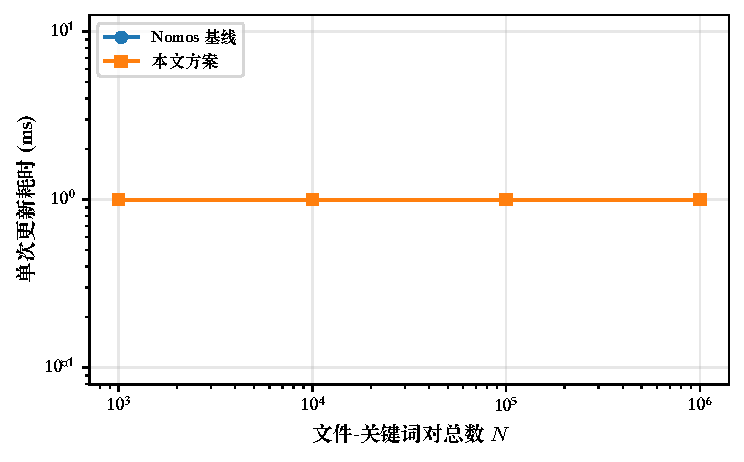
\includegraphics[width=0.85\textwidth]{update-time.pdf}
\caption{不同数据规模下的单次关系更新耗时}
\label{fig:update-time}
\end{figure}

图~\ref{fig:update-breakdown}进一步分解本文方案的更新开销，区分 $\mathsf{QTree}$ 路径更新、承诺计算与基线更新三部分的耗时占比。

\begin{figure}[t]
\centering
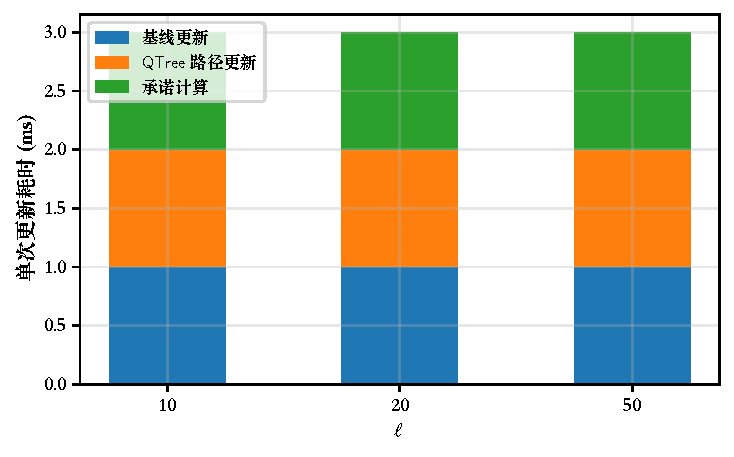
\includegraphics[width=0.85\textwidth]{update-breakdown.pdf}
\caption{更新开销分解（$M=2^{22}$，$N=10^5$）}
\label{fig:update-breakdown}
\end{figure}

\subsection{搜索与证明生成性能}\label{sec:exp-search}

图~\ref{fig:search-time}展示不同候选集规模 $|\mathsf{Cand}(w_s)|$ 下，搜索阶段（含证明生成）的服务器端耗时。

\begin{figure}[t]
\centering
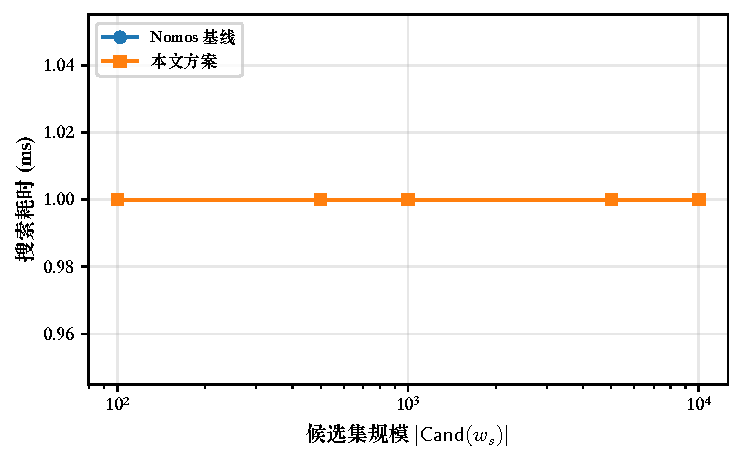
\includegraphics[width=0.85\textwidth]{search-time.pdf}
\caption{不同候选集规模下的搜索耗时（$n=3$，$k=10$，$M=2^{22}$）}
\label{fig:search-time}
\end{figure}

图~\ref{fig:verify-time}展示客户端验证阶段的耗时，包含 $\mathsf{QTree}$ 路径验证与承诺开封验证两部分。

\begin{figure}[t]
\centering
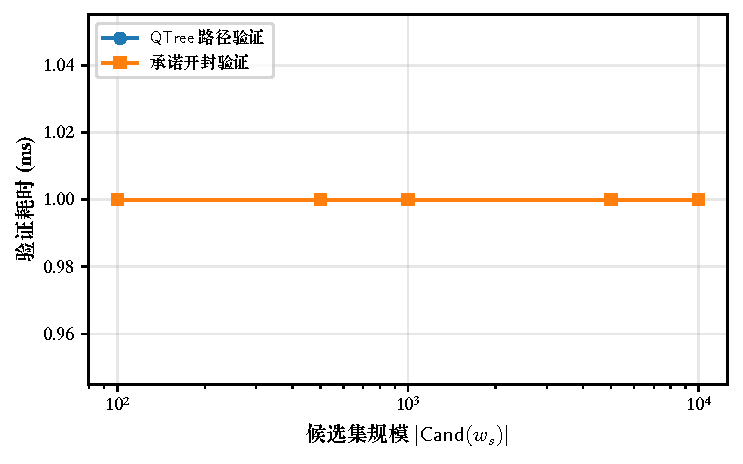
\includegraphics[width=0.85\textwidth]{verify-time.pdf}
\caption{不同候选集规模下的客户端验证耗时（$n=3$，$k=10$）}
\label{fig:verify-time}
\end{figure}

\subsection{通信与存储开销}\label{sec:exp-comm}

图~\ref{fig:comm-overhead}展示不同合取关键词数 $n$ 下，单次查询的通信量对比。

\begin{figure}[t]
\centering
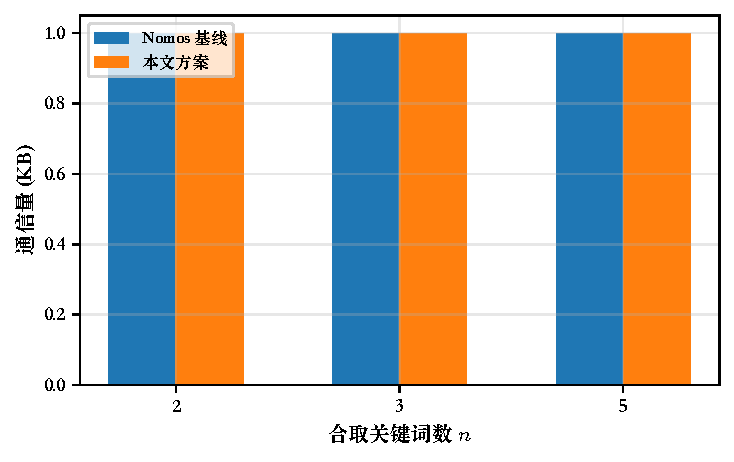
\includegraphics[width=0.85\textwidth]{comm-overhead.pdf}
\caption{不同合取关键词数下的单次查询通信量（$|\mathsf{Cand}|=1000$，$k=10$）}
\label{fig:comm-overhead}
\end{figure}

图~\ref{fig:storage-overhead}展示不同数据规模 $N$ 下，服务器端存储开销对比。

\begin{figure}[t]
\centering
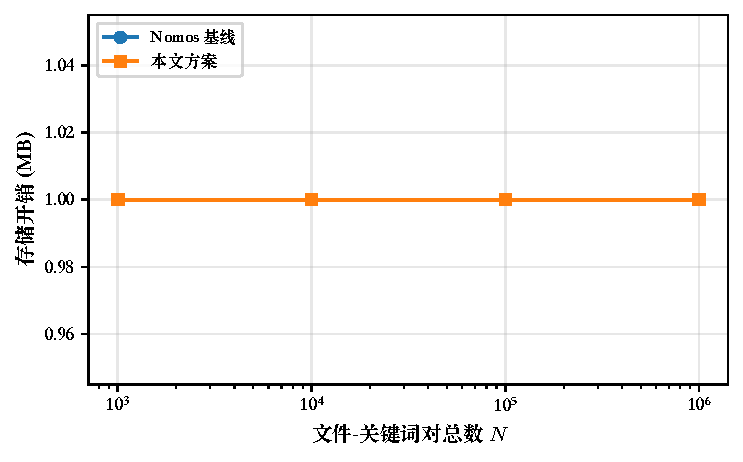
\includegraphics[width=0.85\textwidth]{storage-overhead.pdf}
\caption{不同数据规模下的服务器端存储开销（$\ell=20$，$M=2^{22}$）}
\label{fig:storage-overhead}
\end{figure}

\subsection{参数敏感性实验}\label{sec:exp-sensitivity}

图~\ref{fig:param-ell}展示参数 $\ell$ 对更新耗时与通信量的影响。

\begin{figure}[t]
\centering
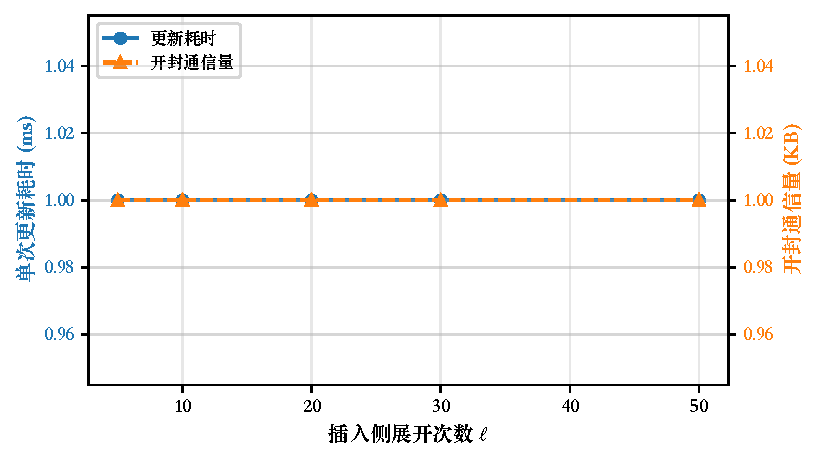
\includegraphics[width=0.85\textwidth]{param-ell.pdf}
\caption{参数 $\ell$ 对更新耗时与开封通信量的影响（$M=2^{22}$，$N=10^5$）}
\label{fig:param-ell}
\end{figure}

图~\ref{fig:param-k}展示参数 $k$ 对证明生成与客户端验证耗时的影响。

\begin{figure}[t]
\centering
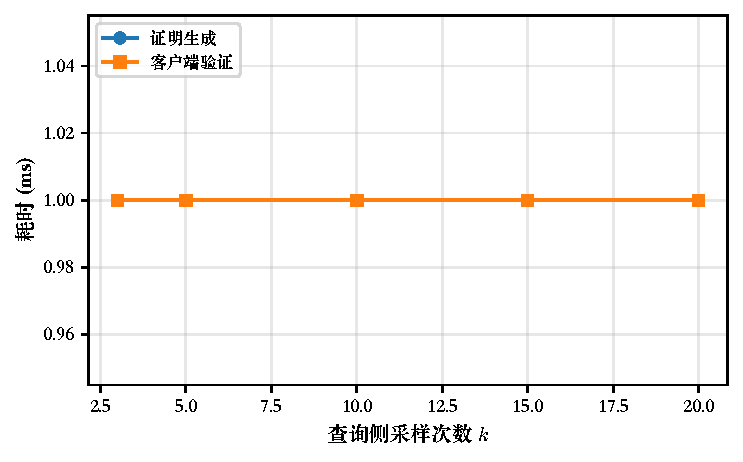
\includegraphics[width=0.85\textwidth]{param-k.pdf}
\caption{参数 $k$ 对证明生成与验证耗时的影响（$|\mathsf{Cand}|=1000$，$n=3$，$M=2^{22}$）}
\label{fig:param-k}
\end{figure}

图~\ref{fig:param-M}展示 $\mathsf{XSet}$ 位数组长度 $M$ 对 $\mathsf{QTree}$ 初始化耗时与单条认证路径长度的影响。

\begin{figure}[t]
\centering
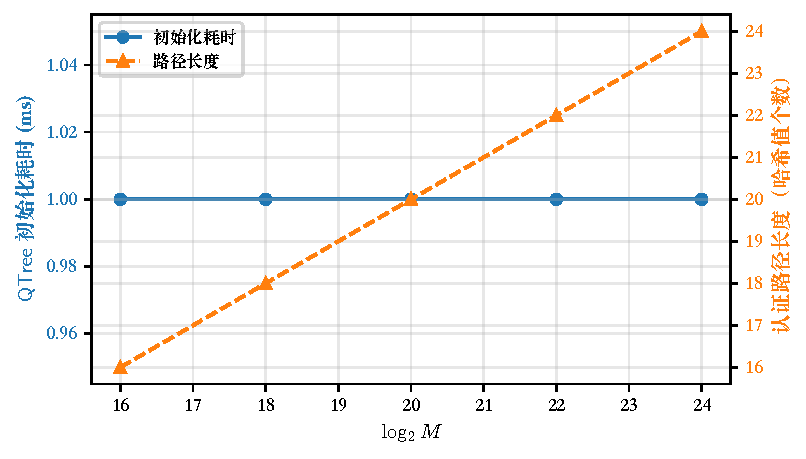
\includegraphics[width=0.85\textwidth]{param-M.pdf}
\caption{$\mathsf{XSet}$ 位数组长度 $M$ 对 $\mathsf{QTree}$ 初始化耗时与路径长度的影响}
\label{fig:param-M}
\end{figure}

\section{本章小结}

本章从渐近复杂度与实验评估两个层面分析了第\ref{chap:bf}章与第\ref{chap:commitment}章提出的可验证机制的开销。理论分析表明，$\mathsf{QTree}$ 的主要增量为 $O(\ell\log M)$ 路径更新与 $O(k\log M)$ 认证路径传输，嵌入式承诺的主要增量为 $O(N\lambda)$ 存储与 $O(\ell\cdot|\mathbb{G}|)$ 开封通信，均为多项式级。实验结果验证了理论预测，并量化了参数 $\ell$、$k$、$M$ 对各阶段性能的影响，为实际部署提供了参数选取依据。


\chapter{总结与展望}

\section{全文总结}
% TODO: 总结全文工作
% 本文面向多用户多关键词对称可搜索加密场景，研究了在泄露受限隐私保护模型下引入轻量可验证机制的问题。
% 主要工作与贡献包括：
%
% 第一，提出了基于 Merkle Hash Tree 的可验证资格检验机制。
% 该机制以 MHT 替换传统 Bloom Filter 组织授权信息，
% 为资格检验结果生成可验证的成员性证明路径，
% 将资格检验从概率判定提升为可证明判断，
% 消除了假阳性导致的错误拒绝风险，
% 并使授权用户能够检测云服务器的选择性作弊行为。
%
% 第二，提出了基于嵌入式承诺的搜索结果正确性验证机制。
% 该机制在数据更新阶段利用承诺机制将校验信息嵌入既有 SSE 索引结构，
% 无需引入独立验证索引，验证开销成为原有索引操作的边际增量。
% 承诺的绑定性保证云服务器无法在搜索阶段伪造与正确结果不一致的校验信息，
% 验证过程在用户端完成，不依赖云服务器的诚实性。
%
% 实验评估表明，两个可验证机制引入后的额外开销处于可接受范围，
% 验证了方案的可行性与工程可落地性。

\section{未来工作展望}
% TODO: 讨论未来研究方向
% - 前向隐私与后向隐私在可验证框架下的联合实现
% - 更丰富的查询语义支持（析取查询、范围查询等）
% - 基于区块链的去中心化可验证搜索
% - 更强对抗模型下的安全性增强（如抗串谋）
% - 面向大规模数据的性能优化与工程实现


%%% 致谢
%%% Local Variables:
%%% mode: latex
%%% TeX-master: "../../main"
%%% End:

\begin{ack}

在硕士研究生经历中，有过许多挑战和成长。回想一路走来，有过研究时的迷惘，有过发表时的兴奋，也有过展望时的徘徊，感慨万千。在此，向所有的支持者表示感谢。
首先，感谢我的导师王婧老师，在研究过程中给予了我无私的指导和支持。王婧不仅在学术上提供了宝贵的建议，还在生活中给予了我关心和鼓励，使我能够顺利完成学业。
其次，感谢我的家人和朋友们，他们一直以来的理解和支持是我坚持下去的动力。无论是在学业上还是生活中，他们都给予了我无尽的爱和鼓励，让我能够克服困难，迎接挑战。
最后，感谢所有参与和支持我研究的人们，包括同学、同门和实验室的成员们。你们的合作和帮助使我的研究工作更加顺利和有意义。
再次感谢所有支持我的人们，你们的帮助和鼓励让我能够完成这段充实而有意义的硕士研究生经历。未来，我将继续努力，不断追求学术上的进步和个人的成长。

\end{ack}



%%% 参考文献
%Included for Gather Purpose only:
%input "ref/refs.bib"
% 注意，中文文献需要在bib条目中任意指定language或者langid为chinese
\bibliographystyle{HUSTThesis}
\bibliography{ref/thesis}

% ---------------------------------------------

%%% 附录
\begin{appendix}
  \begin{publications}

\textbf{学术论文}

\renewcommand{\labelenumi}{[\theenumi]}
\begin{enumerate}
    \item XXX, XXX, \textbf{\underline{XXX}}, XXX, XXX, XXX. FDXT: Forward and Backward Private Conjunctive Searchable Encryption to Suppress Volume Leakages Caused by Cross-Tags. Under major review at \textit{IEEE Transactions on Information Forensics and Security }(TIFS，中科院一区top，CCF A).
\end{enumerate}

\bigskip

\textbf{比赛获奖}
\renewcommand{\labelenumi}{[\theenumi]}
\begin{enumerate}
    \item 第八届全国密码技术竞赛 \hfill 国家级三等奖，队长
\end{enumerate}

\bigskip

\textbf{研究生荣誉}
\renewcommand{\labelenumi}{[\theenumi]}
\begin{enumerate}
    \item 华中科技大学\qquad 学业一等奖学金 \hfill 2023
    \item 华中科技大学\qquad 学业二等奖学金 \hfill 2024，2025
    \item 华中科技大学\qquad 文体公益奖学金 \hfill 2025
\end{enumerate}
\end{publications}
  \chapter{中英文缩写对照表}\label{app:abbr-list}

\begingroup
\footnotesize
\renewcommand{\arraystretch}{1.45}
\begin{center}
\begin{tabularx}{0.92\textwidth}{@{}p{0.18\textwidth}X@{}}
SE & Searchable Encryption（可搜索加密）\\
SSE & Searchable Symmetric Encryption（对称可搜索加密）\\
VSE & Verifiable Searchable Encryption（可验证可搜索加密）\\
PEKS & Public-Key Encryption with Keyword Search（公钥关键词搜索加密）\\
MRSW & Multiple-Reader Single-Writer（多读者单写者）\\
RBF & Redundant Bloom Filter（冗余布隆过滤器）\\
MHT & Merkle Hash Tree（Merkle 哈希树）\\
PRF & Pseudorandom Function（伪随机函数）\\
OPRF & Oblivious Pseudorandom Function（不经意伪随机函数）\\
AE & Authenticated Encryption（认证加密）\\
PPT & Probabilistic Polynomial Time（概率多项式时间）\\
IND-CPA & Indistinguishability under Chosen Plaintext Attack（选择明文攻击下的不可区分性）\\
INT-CTXT & Integrity of Ciphertexts（密文完整性）\\
CRHF & Collision-Resistant Hash Function（抗碰撞哈希函数）\\
CR & Collision Resistance（抗碰撞性）\\
EUF-CMA & Existential Unforgeability under Chosen Message Attack（选择消息攻击下的存在性不可伪造）\\
VQ & Verifiable Qualification（可验证资格检验）\\
\end{tabularx}
\end{center}
\endgroup

\chapter{文中符号一览表}\label{app:symbol-list}

\begingroup
\footnotesize
\setlength{\LTleft}{0pt}
\setlength{\LTright}{0pt}
\renewcommand{\arraystretch}{1.15}
\begin{longtable}{@{}p{0.28\textwidth}p{0.68\textwidth}@{}}
\toprule
符号 & 含义\\
\midrule
\endfirsthead
\toprule
符号 & 含义\\
\midrule
\endhead
\bottomrule
\endfoot
$\lambda$ & 安全参数\\
$\mathsf{negl}(\lambda)$ & 关于安全参数 $\lambda$ 的可忽略函数\\
$\mathbb{G}$ & 素阶 $p$ 的循环群\\
$p$ & 循环群 $\mathbb{G}$ 的素阶\\
$g$ & 循环群 $\mathbb{G}$ 的生成元\\
$F:\{0,1\}^\lambda\times\{0,1\}^*\to\{0,1\}^\lambda$ & 伪随机函数（PRF）\\
$H:\{0,1\}^*\to\{0,1\}^\lambda$ & 抗碰撞哈希函数\\
$F_p:\mathbb{Z}_p^*\times\{0,1\}^*\to\mathbb{Z}_p^*$ & 模 $p$ 伪随机函数\\
$\mathsf{AE}=(\mathsf{AE.Enc},\mathsf{AE.Dec})$ & 认证加密方案\\
$\mathcal{F}_{j,\mathsf{id}}=(\mathsf{xtag}_{j,\mathsf{id}}^{(1)},\ldots,\mathsf{xtag}_{j,\mathsf{id}}^{(\ell)})$ & 候选文件 $\mathsf{id}$ 与非主关键词 $w_j$ 对应的完整地址集合\\
$H_m:\{0,1\}^*\to\{0,1\}^{\lambda}$ & Merkle-Open 认证哈希函数\\
$L_{j,\mathsf{id}}^{(r)}$ & 第 $r$ 个叶子摘要，$L_{j,\mathsf{id}}^{(r)}=H_m(0\|r\|\mathsf{xtag}_{j,\mathsf{id}}^{(r)})$\\
$\mathsf{rt}_{j,\mathsf{id}}$ & 地址集合 $\mathcal{F}_{j,\mathsf{id}}$ 的 Merkle 根\\
$\sigma_{j,\mathsf{id}}$ & $\mathcal{G}$ 对 $(I(w_j)\|\mathsf{rt}_{j,\mathsf{id}})$ 的签名\\
$\mathsf{Auth}_{j,\mathsf{id}}=(\mathsf{rt}_{j,\mathsf{id}},\sigma_{j,\mathsf{id}})$ & 地址集合的根认证对象\\
$\pi_{j,\mathsf{id}}^{(r)}$ & 第 $r$ 个叶子到根 $\mathsf{rt}_{j,\mathsf{id}}$ 的 Merkle 认证路径\\
$\mathsf{Open}_{j,\mathsf{id}}$ & 采样位置的选择性开封材料\\
$\mathsf{VfMPath}(\mathsf{rt},L,\pi)\to\{0,1\}$ & Merkle 路径验证：检查叶子摘要 $L$ 沿路径 $\pi$ 是否归约到根 $\mathsf{rt}$\\
$\mathsf{MPos}$ & 由交叉标签到 $(r,\mathsf{rt},\sigma)$ 的位置映射\\
$\mathsf{MTree}$ & 由根到对应 Merkle 树辅助状态的映射\\
$\mathsf{Proof}_{j,\mathsf{id}}$ & 关系 $(j,\mathsf{id})$ 的 $\mathsf{QTree}$ 资格检验证据\\
$\mathsf{ProofAddr}_{j,\mathsf{id}}$ & $\mathsf{Proof}_{j,\mathsf{id}}$ 中服务器实际声明的物理地址集合\\
\end{longtable}
\endgroup

  \chapter{基础协议实例算法形式化定义}\label{app:base-protocol}

本附录给出第~\ref{subsec:base-protocol} 节所述基础协议实例的四阶段算法伪码，即 Bag 等人\cite{10.1145/3634737.3657018}基于 ODXT\cite{patranabis2021forward} 的动态合取 SSE 构造在初始化、更新、令牌生成与搜索阶段的完整形式化定义。

\begin{breakablealgorithm}
\caption{初始化流程 $\mathsf{Setup}$}
\label{alg:sse-setup}
\begin{algorithmic}[1]
\item[] \textbf{授权管理方:}
\STATE 从 $\mathbb{Z}_p^*$ 中均匀采样随机密钥 $K_S$
\STATE 均匀采样两个随机密钥集合 $K_T=\{K_T^1,\ldots,K_T^d\}$ 与 $K_X=\{K_X^1,\ldots,K_X^d\}$
\STATE 从 $\{0,1\}^{\lambda}$ 均匀采样随机密钥 $K_Y$
\STATE 从 $\{0,1\}^{\lambda}$ 均匀采样随机密钥 $K_M$
\STATE 初始化 $\mathsf{UpdateCnt}\leftarrow\emptyset,\ \mathsf{TSet}\leftarrow\emptyset,\ \mathsf{XSet}\leftarrow\emptyset$
\STATE 授权管理方保留 $\mathsf{sk}=(K_S,K_T,K_X,K_Y)$，按需向客户端披露 $\mathsf{UpdateCnt}$，并由授权管理方与服务器共享 $K_M$，设置 $\mathsf{EDB}=(\mathsf{TSet},\mathsf{XSet})$
\STATE 将 $\mathsf{EDB}$ 发送至服务器
\end{algorithmic}
\end{breakablealgorithm}

\begin{breakablealgorithm}
\caption{更新流程 $\mathsf{Update}$}
\label{alg:sse-update}
\begin{algorithmic}[1]
\item[] \textbf{授权管理方:}
\STATE 解析 $\mathsf{sk}=(K_S,K_T,K_X,K_Y)$ 与 $\mathsf{UpdateCnt}$
\STATE 设置 $K_Z \leftarrow F(H(w)^{K_S},1)$
\STATE 如果 $\mathsf{UpdateCnt}[w]=\mathsf{NULL}$，设置 $\mathsf{UpdateCnt}[w]\leftarrow 0$
\STATE 设置 $\mathsf{UpdateCnt}[w]\leftarrow \mathsf{UpdateCnt}[w]+1$
\STATE 设置 $\mathsf{addr}\leftarrow H(w\|\mathsf{UpdateCnt}[w]\|0)^{K_T[I(w)]}$
\STATE 设置 $\mathsf{val}\leftarrow (\mathsf{id}\|\mathsf{op})\oplus (H(w\|\mathsf{UpdateCnt}[w]\|1))^{K_T[I(w)]}$
\STATE 设置 $\alpha\leftarrow F_p(K_Y,\mathsf{id}\|\mathsf{op})\cdot (F_p(K_Z,w\|\mathsf{UpdateCnt}[w])^{-1})$
\STATE 设置 $\mathsf{xtag}_i\leftarrow H(w)^{K_X[I(w)]\cdot F_p(K_Y,\mathsf{id}\|\mathsf{op})\cdot i}$，$i\in[\ell]$
\STATE 发送 $(\mathsf{addr},\mathsf{val},\alpha,\{\mathsf{xtag}_i\}_{i\in[\ell]})$ 至服务器
\item[] \textbf{服务器:}
\STATE 解析 $\mathsf{EDB}=(\mathsf{TSet},\mathsf{XSet})$
\STATE 设置 $\mathsf{TSet}[\mathsf{addr}]\leftarrow (\mathsf{val},\alpha)$
\STATE 设置 $\mathsf{XSet}[\mathsf{xtag}_i]\leftarrow 1$，$i\in[\ell]$
\end{algorithmic}
\end{breakablealgorithm}

\begin{breakablealgorithm}
\caption{令牌生成流程 $\mathsf{GenToken}$}
\label{alg:sse-gentoken}
\begingroup
\small
\setlength{\algorithmicindent}{1.2em}
\setlength{\columnsep}{1em}
\begin{multicols}{2}
\begin{algorithmic}[1]
\item[] \textbf{客户端:}
\STATE 设置 $m\leftarrow \mathsf{UpdateCnt}[w_1]$（$w_1$ 为最不频繁更新关键词）
\STATE 采样 $r_1,\ldots,r_n \xleftarrow{\$}\mathbb{Z}_p^*$，采样 $s_1,\ldots,s_m \xleftarrow{\$}\mathbb{Z}_p^*$
\STATE 设置 $a_j = H(w_j)^{r_j}$，$j=1,\ldots,n$
\STATE 设置 $b_j = H(w_1\|j\|0)^{s_j}$，$j=1,\ldots,m$
\STATE 设置 $c_j = H(w_1\|j\|1)^{s_j}$，$j=1,\ldots,m$
\STATE 设置 $\mathsf{av}=(I_1,\ldots,I_n)$，其中 $I_j=I(w_j)$
\item[] \textbf{授权管理方:}
\STATE 如果 $\mathsf{av}\notin \mathcal{P}$，终止
\STATE 采样 $\rho_1,\ldots,\rho_n \xleftarrow{\$}\mathbb{Z}_p^*$，采样 $\gamma_1,\ldots,\gamma_m \xleftarrow{\$}\mathbb{Z}_p^*$
\STATE 设置 $\mathsf{strap}' = (a_1)^{K_S}$
\STATE 设置 $\mathsf{bstag}'_j = (b_j)^{K_T[I_1]\cdot \gamma_j}$，$j=1,\ldots,m$
\STATE 设置 $\delta'_j = (c_j)^{K_T[I_1]}$，$j=1,\ldots,m$
\STATE 设置 $\mathsf{bxtrap}'_j = (a_j)^{K_X[I_j]\cdot \rho_j}$，$j=2,\ldots,n$
\STATE 采样 RBF 随机索引 $\beta_i \xleftarrow{\$}[\ell]$，$i\in[k]$
\FOR{$j=2$ to $n$}
  \STATE 初始化 $\overline{\mathsf{bxtrap}}'_j = \emptyset$
  \STATE 更新 $\overline{\mathsf{bxtrap}}'_j = \overline{\mathsf{bxtrap}}'_j\cup\{(\mathsf{bxtrap}'_j)^{\beta_i}\}$，$\beta_i\in\{\beta_1,\ldots,\beta_k\}$
\ENDFOR
\STATE 设置 $\mathsf{env} \leftarrow \mathsf{AE.Enc}_{K_M}(\rho_1,\ldots,\rho_n,$
\item[] \hspace*{\algorithmicindent} $\gamma_1,\ldots,\gamma_m)$
\STATE 设置 $\tau'=(\mathsf{strap}',\{\mathsf{bstag}'_j\}_{j=1}^{m},\{\delta'_j\}_{j=1}^{m},$
\item[] \hspace*{\algorithmicindent} $\{\overline{\mathsf{bxtrap}}'_j\}_{j=2}^{n},\mathsf{env})$
\STATE 发送 $\tau'$ 至客户端
\item[] \textbf{客户端:}
\STATE 设置 $\mathsf{strap} = (\mathsf{strap}')^{r_1^{-1}}$
\STATE 设置 $\mathsf{bstag}_j = (\mathsf{bstag}'_j)^{s_j^{-1}}$，$j=1,\ldots,m$
\STATE 设置 $\delta_j = (\delta'_j)^{s_j^{-1}}$，$j=1,\ldots,m$
\FOR{$j=2$ to $n$}
  \STATE 初始化 $\overline{\mathsf{bxtrap}}_j = \emptyset$
  \STATE 设置 $u_j\leftarrow r_j^{-1}$
    \FOR{$l=1$ to $k$}
      \STATE 设置 $\mathsf{bx}_{j,l}\leftarrow (\overline{\mathsf{bxtrap}}'_j[l])^{u_j}$
      \STATE 更新 $\overline{\mathsf{bxtrap}}_j\leftarrow \overline{\mathsf{bxtrap}}_j\cup\{\mathsf{bx}_{j,l}\}$
    \ENDFOR
\ENDFOR
\STATE 输出 $\tau=(\mathsf{strap},\{\mathsf{bstag}_j\}_{j\in[m]},\{\delta_j\}_{j\in[m]},$
\item[] \hspace*{\algorithmicindent} $\{\overline{\mathsf{bxtrap}}_j\}_{j=2}^{n},\mathsf{env})$
\end{algorithmic}
\end{multicols}
\endgroup
\end{breakablealgorithm}

\begin{breakablealgorithm}
\caption{搜索流程 $\mathsf{Search}$}
\label{alg:sse-search}
\begin{algorithmic}[1]
\item[] \textbf{客户端:}
\STATE 设置 $K_Z \leftarrow F(\mathsf{strap},1)$，设置 $m \leftarrow \mathsf{UpdateCnt}[w_1]$
\STATE 初始化 $\mathsf{stokenList}\leftarrow\emptyset$，初始化 $\mathsf{xtokenList}_1,\ldots,\mathsf{xtokenList}_m\leftarrow\emptyset$
\FOR{$j=1$ to $m$}
  \STATE 更新 $\mathsf{stokenList}=\mathsf{stokenList}\cup\{\mathsf{bstag}_j\}$
  \STATE 设置 $e_j\leftarrow F_p(K_Z,w_1\|j)$
  \FOR{$i=2$ to $n$}
    \STATE 初始化 $\mathsf{xtokenSet}_{i,j}\leftarrow\emptyset$
    \FOR{$t=1$ to $k$}
      \STATE 设置 $\mathsf{xtoken}_{i,j}^{(t)}\leftarrow (\overline{\mathsf{bxtrap}}_i[t])^{e_j}$
      \STATE 更新 $\mathsf{xtokenSet}_{i,j}=\mathsf{xtokenSet}_{i,j}\cup\{\mathsf{xtoken}_{i,j}^{(t)}\}$
    \ENDFOR
    \STATE 随机置换 $\mathsf{xtokenSet}_{i,j}$ 中各元组条目次序
    \STATE 更新 $\mathsf{xtokenList}_j=\mathsf{xtokenList}_j\cup\mathsf{xtokenSet}_{i,j}$
  \ENDFOR
\ENDFOR
\STATE 发送 $(\mathsf{stokenList},\{\mathsf{xtokenList}_j\}_{j=1}^{m})$ 至服务器
\item[] \textbf{服务器:}
\STATE 收到客户端的 $\mathsf{env}$ 后先执行验证；若验证失败则返回 $\bot$，否则解密 $\mathsf{env}$
\STATE 解析 $\mathsf{EDB}=(\mathsf{TSet},\mathsf{XSet})$，初始化 $\mathsf{sEOpList}\leftarrow\emptyset$
\FOR{$j=1$ to $|\mathsf{stokenList}|$}
  \STATE 设置 $\mathsf{cnt}_j\leftarrow 1$
  \STATE 设置 $\mathsf{stag}_j\leftarrow (\mathsf{stokenList}[j])^{1/\gamma_j}$
  \STATE 设置 $(\mathsf{sval}_j,\alpha_j)=\mathsf{TSet}[\mathsf{stag}_j]$
  \FOR{$i=2$ to $n$}
    \STATE 初始化 $\mathsf{flag}\leftarrow 1$
    \STATE 设置 $\mathsf{xtokenSet}_{i,j}\leftarrow \mathsf{xtokenList}_j[i]$
    \FOR{$t=1$ to $k$}
      \STATE 计算 $\mathsf{xtag}_{i,j}\leftarrow (\mathsf{xtoken}_{i,j}^{(t)})^{\alpha_j/\rho_i}$
      \IF{$\mathsf{XSet}[\mathsf{xtag}_{i,j}]=0$}
        \STATE 设置 $\mathsf{flag}\leftarrow 0$
      \ENDIF
    \ENDFOR
    \IF{$\mathsf{flag}=1$}
      \STATE 设置 $\mathsf{cnt}_j\leftarrow \mathsf{cnt}_j+1$
    \ENDIF
  \ENDFOR
  \STATE 设置 $\mathsf{sEOp}_j\leftarrow (j,\mathsf{sval}_j,\mathsf{cnt}_j)$
  \STATE 更新 $\mathsf{sEOpList}\leftarrow \mathsf{sEOpList}\cup\{\mathsf{sEOp}_j\}$
\ENDFOR
\STATE 将 $\mathsf{sEOpList}$ 发送至客户端
\item[] \textbf{客户端:}
\STATE 初始化 $\mathsf{IdList}\leftarrow\emptyset$
\FOR{$c=1$ to $|\mathsf{sEOpList}|$}
  \STATE 令 $(j,\mathsf{sval}_j,\mathsf{cnt}_j)=\mathsf{sEOpList}[c]$
  \STATE 恢复 $(\mathsf{id}_j\|\mathsf{op}_j)=\mathsf{sval}_j\oplus\delta_c$
  \IF{$\mathsf{op}_j=\mathsf{DEL}\land \mathsf{cnt}_j=n$}
    \STATE 设置 $\mathsf{IdList}=\mathsf{IdList}\setminus\{\mathsf{id}_j\}$
  \ENDIF
\ENDFOR
\STATE 输出 $\mathsf{IdList}$
\end{algorithmic}
\end{breakablealgorithm}

\end{appendix}

\end{document}
